\documentclass[12pt]{n-te}

\usepackage{dblfloatfix}
\usepackage[pdftitle={Erstsemesterzeitung der Fachgruppe Informatik WS08/09},pdfauthor={Fachgruppe Informatik}]{hyperref}
%\usepackage[latin1]{inputenc}
\usepackage{
  floatflt,
  graphicx,
  ngerman,
  pdfpages,
  subfig,
  subfloat,
  units,
  wasysym
}

\nedition{1}{WS 2008/2009}

%% Trennregeln
\hyphenation{AStA}
\hyphenation{Mit-be-wohnerIn-nen}
\hyphenation{Pro-fessorInnen}
\hyphenation{erwischt}
\hyphenation{viiieel}
\hyphenation{y-Nummer}
\hyphenation{Uniaccount}
%\hbadness=10000

\begin{document}
  \begin{titlepage}
  \setlength{\topmargin}{-24mm}
  \setlength{\headheight}{0pt}
  \begin{figure}[t]
    \includegraphics[bb=20mm 0mm 200mm 287mm]{bilder/titelseite.png}
  \end{figure}
  \thispagestyle{empty}
  \newpage
\end{titlepage}


  \setcounter{page}{1}
  \begin{figure*}[t]
    \includegraphics[height=\textheight]{bilder/lageplan.png}
  \end{figure*}
  \clearpage

  
\section{Vorwort}
\label{vorwort}
	\begin{multicols}{2}
	\subsection*{Willkommen in der Informatik!}	

	Ein neues Semester hat begonnen und wieder strömen unzählige neue Gesichter auf den Campus um das Abenteuer Studium zu beginnen oder fortzusetzen. Da das nicht immer ganz einfach ist haben wir, die Fachgruppe Informatik für die Erstsemester unserer Fachrichtung einen kleinen Leitfaden zusammengestellt - die 1-te.

	Auf den folgenden Seiten werden wir hoffentlich einige der typischen Fragen beantworten, die einen am Anfang des Studiums quälen. Außerdem möchten wir natürlich uns, die Fachgruppe vorstellen (s. Seite \pageref{fachgruppe}) und eventuell noch die ein oder andere hilfreiche Information mitgeben. 

	\subsubsection*{Aufbau dieses Heftes}
		In der ersten Hälfte dieses Heftes sind wichtige
		Erklärungen zum Studienbeginn, dem Studiengang und der
		universitären Infrastruktur. Weitere Informationen zu
		uns und unserer Gremienarbeit, sowie weitere
		Informationen sind in der zweiten Hälfte.
\columnbreak
	\subsubsection*{Die Fachgruppe Online}
		Natürlich gibt es uns auch online - auf der Seite \url{http://fginfo.cs.tu-bs.de}. Beispielsweise stehen dort aktuelle Termine wie Spiele- oder Grillabende. Auch gibt es dort noch einmal die Inhalte dieses Heftes, samt den Aktualisierungen die erst nach dem Druck bekannt wurden. 

	\vspace*{0.5cm}

	Viel Spaß und Erfolg im  Studium wünscht  die\\
	\hspace*{2cm}Fachgruppe Informatik
	\end{multicols}
	\vspace{0.5cm}
	\begin{center} 
\includegraphics[totalheight=12cm]{bilder/XKCD/dorm_poster}
\end{center}

  \newpage
  \ntoc %% Inhaltsverzeichnis
  \clearpage

  \section{Termine}

Gerade in der Anfangszeit des Studiums gibt es eine Menge zu tun. Damit ihr
nicht das Wichtigste verpasst, haben wir die ersten Termine kompakt f"ur
euch zusammengefasst. Die meisten davon bieten die Gelegenheit Fragen zu
stellen und nebenbei gleich ein paar nette Kommilitonen kennen zu lernen.

In der \textit{Ort}-Spalte stehen meist Raumnummern. F"ur alle R"aume die nicht
im IZ (steht f"ur Informatikzentrum) liegen, schaut am besten auf den
Campusplan im Einband. Bei den R"aumen im IZ ist die erste Zahl das Stockwerk, f"ur
den Rest m"usst ihr dann auf den Plan im Stockwerk schauen (Kleine Falle:
zwischen EG und 1. OG liegt das Galeriegescho"s - Raum IZ 150 liegt also
effektiv in der zweiten Etage). \par

\begin{figure}[h]
\begin{tabular}{|l|l|p{6.7cm}|c|c|c|}
\hline \textbf{Datum} & \textbf{Uhrzeit} & \textbf{Veranstaltung}	& \textbf{Ort} & \textbf{B} & \textbf{M} \\
\hline 20.10. – 1.10.
				& 1. Tag: 10:00	 & Vorkurs Informatik					& PK 2.2		&B& \\
\hline 11.10. – 22.10. 
				&	 	 		 & Vorkurs Mathematik 					&				&B& \\
\hline 21.10.
				& 10:00 – 11:00	 & Einführung (M) \newline durch die Professoren	& IZ 160/161	& &M\\
\hline 			& 11:15 – 12:45	 & Einführung (M) der Fachgruppe		& IZ 161		& &M\\
\hline 			& 13:00 – 14:30	 & Gemeinsames Stundenplan-Bauen		& IZ 161		& &M\\
\hline 25.10.	&  9:00 – 10:00	 & Begrüßung							& Audimax		&B&M\\
\hline 			& 10:00 – 12:00	 & Infobörse							& Altgebäude	&B&M\\
\hline 			& 13:30 – 15:00	 & Einführung (B) \newline durch die Professoren	& IZ 160/161	&B& \\
\hline 			& 15:00 – 16:30	 & Erste Vorlesung Programmieren		& SN 19.1		&B& \\
\hline 26.10.	& 10:00 – 11:45	 & Ersti-Frühstück						& IZ Plaza		&B&M\\
\hline 			& 12:00 – 13:30	 & Einführung (B) der Fachgruppe		& IZ 161		&B& \\
\hline 			& 12:00 – 14:00	 & Rundgang (M) \newline mit der Tutorengruppe	& IZ 150		& &M\\
\hline 			& 13:30 – 15:30	 & Rundgang (B) \newline mit der Tutorengruppe	& IZ 150		&B& \\
\hline 			& 19:00 – \ldots & Grillen mit der Fachgruppe			& Gaußpark		&B&M\\
\hline 27.10.	& 10:00 – 17:00	 & Studium Generale						& Altgebäude	&B&M\\
\hline 05.11.	& 19:00 – \ldots & Kneipentour mit der Fachgruppe		& IZ 150		&B&M\\
\hline 10.11.	& 16:30 – \ldots & Spieleabend der Fachgruppe			& vor IZ 150	&B&M\\ 
\end{tabular} 
\end{figure}

\newpage

% - Gl"uhweinabend im Informatikzentrum (IZ)

  \section{Gruppen}
% !TEX root = ../../1-te.tex

\subsection{Fachgruppe}
	\label{fachgruppe}
%	\fginfoUrl
	Die Fachgruppe seid ihr! Die Fachgruppe aus allen Studierenden der Fachrichtung Informatik. Diese wählen einen Fachgruppenrat, der sich dann für die Interessen aller einsetzt. 
	Im Fachgruppenraum IZ150 stehen dir jederzeit zuverlässige Mitstudierende zur Verfügung, denen du Fragen bezüglich deines Studiums und allem drumherum stellen kannst. Einige sind Mitglieder des Fachgruppenrats und dafür verantwortlich, die Meinungen aller Informatikstudierenden gegenüber der Fakultät und in verschiedenen Kommissionen zu vertreten. Eine richtige Trennung zwischen Fachgruppenrat und Fachgruppe besteht bei uns nicht. Also komm vorbei, bring dich ein und engagier dich für unsere Studienrichtung oder hol dir einfach ein paar koffeinreiche Erfrischungen. 

\subsection{Tutorien}
Da der Einstieg ins Studium alleine relativ schwierig ist und sich viele Fragen in einer Gruppe am einfachsten beantworten lassen, gibt es Tutorengruppen, denen du am Montag um ca. 15 Uhr zugeteilt wirst. 
In diesen findet dann ein Rundgang über den Campus und die wichtigsten Einrichtungen in der Nähe statt. 
Dort hast du außerdem die Möglichkeit in überschaubarer Runde andere Informatikstudenten und eben eure Tutoren kennen zu lernen, sowie weitere Informationen zu deinen Veranstaltungen und Dozenten zu erhalten.
Scheu dich nicht, einen der Tutoren zu kontaktieren. Da weitere Treffen geplant sind kannst du dich auch nachträglich noch in eine Tutorengruppe einteilen lassen. Dazu schreibt bitte eine Mail an die Fachgruppe \url{fginfo@tu-bs.de} oder direkt an einen der Tutoren.


\ifpdf
Damit du schonmal das ein oder andere Gesicht kennst, sind hier die Fotos der Tutoren abgebildet.
%%
\end{multicols}



% TODO Bilder aktualisieren, angeben, ob der jenige Bachelors oder Masters betreut (ist ja nicht immer identisch damit, was man selbst gerade ist)
% NICHT als \paragraph, da das leider das Layout verhaut. Ist natürlich
% unschön ):
%Leider ist das ganze Layout etwas screwed
%Also ein alter Trick aus Web 1.0 Tagen\ldot.
%Layout Tabellen! Nicht schön, aber wenns sonst nicht geht\ldot.
  \begin{tabular}{c}
\begin{tabular}{lll}
  { \textbf{Bachelor Tutoren}} \ \\ 
% \picture[0.3\linewidth]
% {bilder/tutoren/kris.jpg}
% {Christoph\\ 3. Semester Master\\ \randomize{admin@keeg.de}}
% \ {
{
\picture[0.3\linewidth]
{bilder/tutoren/dominik_pass}
{Dominik\\%3. Semester Master\\ 
\randomize{d.schuermann@tu-bs.de}}
}%\hfill
& \ 
%{\picture[2.3\linewidth]
%{bilder/tutoren/franziska.jpg}
%{Franziska\\6. Semester Bachelor\\ \randomize{f.werk@tu-bs.de}}
%}%\\ \ \\
{\picture[0.3\linewidth]
{bilder/tutoren/jan_germann.jpg}
{Jan\\%2. Semester Bachelor\\ 
\randomize{j.germann@tu-bs.de}}
} 
&\
{
\picture[0.3\linewidth]
{bilder/tutoren/hf}
{Hella\\% 2. Semester Master\\ 
\randomize{h-f.hoffmann@tu-bs.de}}}
\\ \  \\
%\hfill
{\picture[0.3\linewidth]
{bilder/tutoren/johannes.jpg}
{Johannes\\% 7. Semester Bachelor\\ 
\randomize{J.Starosta@tu-bs.de}}
}& \ 
%\hfill
% {\picture[0.3\linewidth]
% {bilder/tutoren/judith.jpg}
% {Judith\\ 5. Semester Bachelor\\ \randomize{judith.hilpert@web.de}}}\\
% \ \\
% \picture[0.3\linewidth]
% {bilder/tutoren/marekd.jpg}
% {Marek\\ 1. Semester Master\\ \randomize{m.drogon@tu-bs.de}}
% &  %\hfill
 {
 \picture[0.3\linewidth]
 {bilder/tutoren/sebastian.jpeg}
 {Sebastian\\ %9. Semester Bachelor\\ 
\randomize{se.busse@tu-bs.de}}} 
%&{
%\picture[0.3\linewidth]%{}
%{bilder/tutoren/serj}
%{Serj\\ 1. Semester Master\\\randomize{s.dechand@tu-bs.de }}}
%\par \ \par  
%\end{tabular}
%
%\begin{center}
%  \begin{tabular}{ccc}
 %    { \picture[0.3\linewidth]%{}
 % {bilder/tutoren/christina}
 % {Christina\\ 5. Semester Bachelor\\\randomize{c.eberth@tu-bs.de}}}
%{
%\picture[0.3\linewidth]%{}
%{bilder/tutoren/viktor}
%{Viktor Richert\\ 4. Semester Bachelor\\%}%\\ 5. Semester Bachelor\\
%\randomize{InformatikWiki@gmx.de}}%.eberth@tu-bs.de }
% }&{
%  \picture[0.3\linewidth]%{}
%  {bilder/tutoren/dummy}
%  {Christoph\\ 5. Semester Bachelor\\ \randomize{christoph.harburg@web.de}}
% }\\
&\ {\picture[0.3\linewidth]%{}
{bilder/tutoren/joko_n}
{Jonathan\\% 7. Semester Bachelor \\
\randomize{j.koscielny@tu-bs.de}}}
\\ \  \\
{\picture[0.3\linewidth]%{}
{bilder/tutoren/viktor}
{Viktor\\% 5. Semester Bachelor\\%\\ 5. Semester Bachelor\\
\randomize{InformatikWiki@gmx.de}}}
&\ {\picture[0.3\linewidth]%{}
{bilder/tutoren/rcfinster_sm}
{Rebecca \\ % Bachelor\\%}%\\ 5. Semester Bachelor\\
\randomize{r.finster@tu-bs.de}}}
& \ 
{\picture[0.3\linewidth]
{bilder/tutoren/keno_sw.jpg}
{Keno\\%2. Semester Bachelor\\ 
\randomize{k.garlichs@tu-bs.de}}
}
\end{tabular}%\tabularnewline \\
\end{tabular}\tabularnewline \\
%\begin{left}
\newpage
%\begin{center}
\begin{tabular}{ccc}
{ \textbf{Master Tutoren}}\\
% NICHT als \paragraph, da das leider das Layout verhaut. Ist natürlich
% unschön ):
\picture[0.3\linewidth]
{bilder/tutoren/martinw_sw.jpg}
{Martin\\% 4. Semester Master\\ 
\randomize{m.wegner@tu-bs.de}}
&
%{ 
%\picture[0.3\linewidth]
%{bilder/tutoren/jan.jpg}
%{Till\\  Master\\ \randomize{t.lorentzen@tu-bs.de}
%}&
%\\
%\hfill %\par \ \par
%{
%\picture[0.3\linewidth]
%{bilder/tutoren/henning.jpg}
%{Henning\\ 5. Semester Master\\ \randomize{h.guenther@tu-bs.de}}
%}&
{ 
\picture[0.3\linewidth]
{bilder/tutoren/sophia.jpg}
{Sophia\\% 3. Semester Master\\
\randomize{s.scholtka@tu-braunschweig.de}}
}
&
{
\picture[0.3\linewidth]%{}
{bilder/tutoren/serj}
{Serj\\% 2. Semester Master\\
\randomize{s.dechand@tu-bs.de }}}
\\ \ \\
{\picture[0.3\linewidth]
{bilder/tutoren/lena_sm.jpg}
{Lena\\ %5. Semester Master\\ 
\randomize{dielenamaria@gmail.com}}
}&
%\hfill
%{\picture[0.3\linewidth]
%{bilder/tutoren/hashier.jpg}%Christopher Lössl < c.loessl@tu-bs.de>
%{Chris \\3. Semester Master\\ \randomize{c.loessl@tu-bs.de}}
%}%&
{\picture[0.3\linewidth]
{bilder/tutoren/till_sw}
{Till\\ %\\  4. Semester Master\\
\randomize{t.lorentzen@tu-bs.de}}
}
%\picture[0.3\linewidth]
%{bilder/tutoren/stephan.jpg}
%{Stephan\\ 5. Semester Master\\ stephan.friedrichs@tu-bs.de}
  \end{tabular}
%  \end{tabular}
  
%\end{center}
\else
In der Druckfassung wären hier die Tutoren mit Emailadresse und Foto aufgelistet. Um die Privatspäre der Tutoren zu schützen, stehen diese jedoch nicht direkt hier in der Onlinefassung.
\fi

%%
%
\begin{multicols}{2}
% Local Variables: 
% mode: latex
% TeX-master: "../../1-te"
% End: 

\onecolumn
\begin{figure}[t]
  %\includegraphics{bilder/gremienkunde.pdf}
  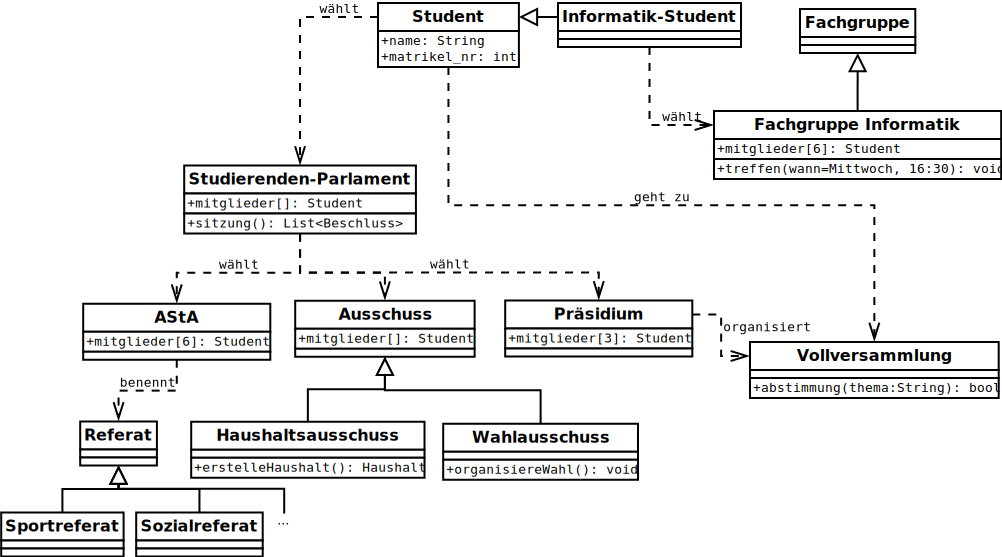
\includegraphics[width=\textwidth]{bilder/gremienkunde2.png}
  \caption{UML Diagramm der Studentischen Selbstverwaltung}
\end{figure}
\twocolumn
\subsection{Studentische Selbstverwaltung f"ur Dummies}
Seit die '68er durch die deutschen Universit"aten gefegt sind, ist Demokratie eingekehrt.
Doch was bedeutet das konkret f"ur euch?
\subsubsection*{Studierendenparlament}
Eines der wichtigsten Elemente der studentischen Mitbestimmung ist das Studierendenparlament (Uni-Slang: StuPa).
Es wird jedes Semester gew"ahlt und entscheidet unter anderem "uber den studentischen Haushalt, den ihr als Teil des Semesterbeitrags zahlt.
Au"serdem werden hier Aussch"usse gew"ahlt (Als wichtigster der "`Allgemeine Studierenden Ausschuss"', kurz AStA).
\subsubsection*{AStA}
Der Allgemeine Studierenden Ausschuss ist die "`Exekutive"' der Studenten:
Er vertritt euch nach Au"sen, also zum Beispiel bei Verhandlungen um das Semesterticket, versorgt euch mit Informationen zu politischen Themen ("ofter im Semester erscheint der so genannte "`AStA-Issue"') und ist einer der ersten Ansprechpartner f"ur eure Anliegen.
\subsubsection*{Fachgruppe}
Auch die Fachgruppe wird von euch gew"ahlt.
Allerdings w"ahlt hier jede Fachrichtung ihre eigene, ihr also Fachgruppe Informatik.
Die Fachgruppe unterst"utzt euch bei Infomatik-spezifischen Fragen, organisiert Veranstaltungen, wie zum Beispiel eure Erstsemester-Einf"uhrung und vertritt euch in verschiedenen Gremien.
\subsubsection*{Gremien}
In der Uni gibt es unz"ahlige Gremien, hier seien die wichtigsten genannt.
Jedes Gremium hat eine bestimmte Besetzung, also eine definierte Anzahl von jeweils Studenten, Mitarbeitern und Professoren.
Am relevantesten für euch ist die Studienkommission (\emph{StuKo}):
Hier werden Details des Studiengangs besprochen, Probleme der Studenten gekl"art und die Vergabe der Studiengebühren entschieden.
In diesem Gremium herrscht ein Stimmengleichgewicht zwischen Studenten und Professoren.
Das bedeutet, dass wir hier wirklich die M"oglichkeit haben, aktiv in die Unipolitik einzugreifen.

In der \emph{Informatik-Kommission} und im \emph{Fakult"atsrat} (der außerdem noch Mitglieder aus der Mathematik hat) sieht es da schon schlechter aus, die Studenten stellen in beiden nur eine Minderheit der Stimmen.

Die \emph{Berufungskommission} hat nur selten zu tun:
Wann immer eine Professur besetzt werden muss, tagt sie um Kandidaten f"ur das Amt zu finden.

Wann immer ihr Antr"age im Pr"ufungsamt stellt, landen diese im \emph{Pr"ufungsausschuss}, der entscheidet, ob diese rechtm"a"sig sind.
In diesem sind drei Professoren, ein Student und ein Mitarbeiter vertreten.

\subsection*{Vollversammlung}
Mindestens einmal im Semester findet eine Vollversammlung aller Studenten statt.
Nehmen genug Studenten teil, so k"onnen hier wichtige Themen abgestimmt werden, die alle Studenten betreffen, zum Beispiel wurde die Einf"uhrung des Semestertickets hier beschlossenx.
  \section{Euer Studienplan}
\subsection{Begriffserklärungen}

% \begin{figure*}[b]
% 	\centering\includegraphics[width=0.9\textwidth]{bilder/comics/wondermark003.png}
% \end{figure*}

% TODO sind die Begriffe, die man für den Studienplan braucht, hier gut untergebracht oder sollten die mit in den restlichen Erklärungstext? Ist das hier wirklich eine kurze, neutrale Begriffserklärung oder nicht eher ein Kapitel "Kritische Kommentrare zu den Vorlesungen und Übungen"?

Einen guten überblick über die an der Uni gebräuchlichen Begriffe und
Abkürzungen findest du im "`Uni-ABC"' des AStA-Erstiinfos. Im folgenden
sind nur die wichtigen Begriffe für deinen Stundenplan erklärt, den du
auf der letzten Seite dieses Heftes findest.




% TODO Spätestens hier (Noch Fragen?) hört's auf, die Fragen sind keine Begriffsklärung mehr. Das ist ja gut, dass es solche Texte gibt, aber die Überschrift passt einfach nicht.
\subsubsection*{Noch Fragen?}

Die Qualität dieser drei Veranstaltungsarten ist in starkem Maße vom
jeweiligen Vortragenden abhängig. Während du unter Umständen die
Seminargruppen noch wechseln kannst, so ist das bei den erstgenannten
Veranstaltungen natürlich nicht möglich.

Du wirst sehr bald feststellen, dass es verschiedene Lerntypen gibt. Manche
deiner Kommilitonen werden kaum eine Vorlesung besuchen, sondern stattdessen die großen
und kleinen übungen verschlingen. Wieder andere lassen sich sowieso kaum im
Hörsaal blicken, sondern können am besten zu Hause oder in der Uni-Bibliothek
autodidaktisch lernen.

Wenn trotz Vorlesungen, großer übungen und kleiner übungen noch Fragen
auftreten, so hilft dir das Gespräch mit den Kommilitonen oder der Blick in
entsprechende Literatur.
Wichtig: Kaufe nicht gleich jedes empfohlene Buch neu,
das ist Geldverschwendung. Frage höhere Semester nach wirklich sinnvoller
Literatur, leih' dir die Bücher aus der UB aus, gebrauchte Bücher gibt es
günstig z.B. in der Newsgroup \url{http://groups.google.de/group/braunschweig.kaufrausch/} (siehe den Artikel
ab Seite \pageref{elekinf}). An der Uni wird man nicht umsorgt wie etwa in der
Schule oder in der betrieblichen Ausbildung, du trägst ein wesentlich höheres
Maß an Eigenverantwortung. Zur Orientierung in der ersten Zeit ist ein
Ansprechpartner unentbehrlich. Wenn die Kommilitonen aus
deinem eigenen Semester nicht weiterhelfen können, dann vielleicht dein/e TutorIn oder andere
Studierende im höheren Semester (zum Beispiel Mitbewohner, Fachgruppe).

\section{Euer Studienplan}
\subsection{Begriffserklärungen}

% \begin{figure*}[b]
% 	\centering\includegraphics[width=0.9\textwidth]{bilder/comics/wondermark003.png}
% \end{figure*}

% TODO sind die Begriffe, die man für den Studienplan braucht, hier gut untergebracht oder sollten die mit in den restlichen Erklärungstext? Ist das hier wirklich eine kurze, neutrale Begriffserklärung oder nicht eher ein Kapitel "Kritische Kommentrare zu den Vorlesungen und Übungen"?

Einen guten überblick über die an der Uni gebräuchlichen Begriffe und
Abkürzungen findest du im "`Uni-ABC"' des AStA-Erstiinfos. Im folgenden
sind nur die wichtigen Begriffe für deinen Stundenplan erklärt, den du
auf der letzten Seite dieses Heftes findest.




% TODO Spätestens hier (Noch Fragen?) hört's auf, die Fragen sind keine Begriffsklärung mehr. Das ist ja gut, dass es solche Texte gibt, aber die Überschrift passt einfach nicht.
\subsubsection*{Noch Fragen?}

Die Qualität dieser drei Veranstaltungsarten ist in starkem Maße vom
jeweiligen Vortragenden abhängig. Während du unter Umständen die
Seminargruppen noch wechseln kannst, so ist das bei den erstgenannten
Veranstaltungen natürlich nicht möglich.

Du wirst sehr bald feststellen, dass es verschiedene Lerntypen gibt. Manche
deiner Kommilitonen werden kaum eine Vorlesung besuchen, sondern stattdessen die großen
und kleinen übungen verschlingen. Wieder andere lassen sich sowieso kaum im
Hörsaal blicken, sondern können am besten zu Hause oder in der Uni-Bibliothek
autodidaktisch lernen.

Wenn trotz Vorlesungen, großer übungen und kleiner übungen noch Fragen
auftreten, so hilft dir das Gespräch mit den Kommilitonen oder der Blick in
entsprechende Literatur.
Wichtig: Kaufe nicht gleich jedes empfohlene Buch neu,
das ist Geldverschwendung. Frage höhere Semester nach wirklich sinnvoller
Literatur, leih' dir die Bücher aus der UB aus, gebrauchte Bücher gibt es
günstig z.B. in der Newsgroup \url{http://groups.google.de/group/braunschweig.kaufrausch/} (siehe den Artikel
ab Seite \pageref{elekinf}). An der Uni wird man nicht umsorgt wie etwa in der
Schule oder in der betrieblichen Ausbildung, du trägst ein wesentlich höheres
Maß an Eigenverantwortung. Zur Orientierung in der ersten Zeit ist ein
Ansprechpartner unentbehrlich. Wenn die Kommilitonen aus
deinem eigenen Semester nicht weiterhelfen können, dann vielleicht dein/e TutorIn oder andere
Studierende im höheren Semester (zum Beispiel Mitbewohner, Fachgruppe).

\section{Euer Studienplan}
\input{texte/studienplan/begriffe}
\input{texte/studienplan/studienplan}
\onecolumn
\begin{figure}[h]
  \centering\includegraphics[angle=90,totalheight=\textheight, width=\textwidth ]{texte/studienplan/studienplan.pdf}
\end{figure}
\twocolumn
\input{texte/studienplan/bpo}
\onecolumn
\begin{figure}[h]
  \centering\includegraphics[angle=90,totalheight=\textheight, width=\textwidth ]{texte/studienplan/studienplan_neu.pdf}
\end{figure}
\twocolumn
\input{texte/studienplan/module}

\onecolumn
\begin{figure}[h]
  \centering\includegraphics[angle=90,totalheight=\textheight, width=\textwidth ]{texte/studienplan/studienplan.pdf}
\end{figure}
\twocolumn
\subsection{Die Prüfungsordnung}
\label{po}
	An einer Universität gibt es tausende Regeln und Ordnungen. Die wichtigste ist die Prüfungsordnung: Sie enthält Antworten auf 95\% aller Fragen, die im Studium auftreten - nicht nur wenn es um die eigentlichen Prüfungen geht. Die genaue Bezeichnung lautet \emph{Besonderer Teil der Prüfungsordnung für den (Bachelor-/Master-)studiengang Informatik der Technischen Universität Braunschweig}. Und da sie weder besonders lang, noch kompliziert geschrieben ist, sollte jeder Student sie einmal überfliegen.

	Außerdem gibt es noch die APO, die Allgemeine Prüfungsordnung. Sie gilt uniweit für alle Studiengänge, doch die beiden BPOs überschreiben die meisten APO-Regelungen.

	Wenn du es noch nicht getan hast, lade dir deine aktuelle Prüfungsordnung am besten von \url{http://www.tu-braunschweig.de/fk1/service/informatik/dokumente} herunter. 



\onecolumn
\begin{figure}[h]
  \centering\includegraphics[angle=90,totalheight=\textheight, width=\textwidth ]{texte/studienplan/studienplan_neu.pdf}
\end{figure}
\twocolumn
% !TEX root = ../../1-te.tex

\subsection{Module und Co.}
	Um deinen Abschluss zu bekommen, musst du eine vordefinierte Menge von Modulen abdecken. Ein Modul besteht aus verschiedenen Bestandteilen.

\subsubsection{Vorlesung, Übung, etc.}
	\paragraph*{Vorlesung}
	Vorlesungen werden vor allen Studis abgehalten und befassen sich in erster Linie mit der theoretischen Herleitung des Stoffes. Solltest du in der Vorlesung einmal etwas nicht verstehen, so ist das nicht so tragisch. Vorlesungen an der Uni unterscheiden sich stark vom Unterricht an der Schule. Gehe nicht davon aus, Vorlesungsinhalte direkt zu verstehen. Plane eine gewisse Nachbearbeitungszeit für die Vorlesungen ein. In einer Vorlesung ist wegen der großen Teilnehmerzahl normalerweise kein Dialog mit dem oder der Vortragenden möglich. Aufgetretene Fragen können und sollten am besten direkt nach der Vorlesung oder sonst in einer Sprechstunde mit der oder dem Lehrenden geklärt werden.
	
	\paragraph*{Große Übung}
	Ergänzend gibt es die großen Übungen, auch Saalübungen genannt. Diese finden, wie die Vorlesung, vor dem gesamten Auditorium statt und sollen das erworbene, theoretische Wissen vertiefen und vor allem auch praktische, klausurbezogene Anwendungen aufzeigen. Die große Übung wird normalerweise von einer Mitarbeiterin oder einem Mitarbeiter gehalten. Sie sind bei  fachlichen Fragen kompetente Ansprechpartner/innen und meistens auch sehr hilfsbereit. Da sie  üblicherweise die Klausuren entwerfen, kann man bei genauem Hinhören in den großen Übungen oder im privaten Gespräch mit ihnen einiges über die Prüfung erfahren.

	\paragraph*{Kleine Übung, Seminargruppe}
	Als erstes eine Warnung: Kleine Übungen tauchen im Stundenplan nicht immer auf und werden leider nur in einigen Fächern angeboten. Der Begriff Seminargruppe ist synonym zu verstehen.
	
	In kleinen Übungen soll man selbst Aufgaben lösen. Dies geschieht unter Anleitung der HiWis (Hilfswissenschaftler/innen), welche meist Studierende höheren Semesters sind. Für die kleinen Übungen werden die Studis in etwa 20- bis 30-köpfige Gruppen aufgeteilt. Hierbei ist darauf zu achten, rechtzeitig zum Termin der Gruppeneinteilung zu erscheinen, um diese Veranstaltungen möglichst günstig im Stundenplan positionieren zu können. Der Termin wird meistens in der ersten Vorlesung bzw. großen Übung bekannt gegeben oder steht auf der jeweiligen Institutsseite. Aufgrund der geringen Teilnehmerzahlen ist in kleinen Übungen der Dialog mit der oder dem Vortragenden möglich und sinnvoll. Bei guten HiWis kann man in den kleinen Übungen all die Wissenslücken auffüllen, die nach Vorlesung und großer Übung offen sind.
	
	\paragraph*{Klausur}
	Klausuren sind schriftliche Prüfungen und finden in nahezu allen Pflichtfächern im Bachelor statt. Man kann sich noch bis 12:00 Uhr des vorherigen Werktags von einer schriftlichen Prüfung abmelden, online sogar bis 23:59 Uhr. Nach Bekanntgabe des Ergebnisses (im Regelfall nach 2-4 Wochen) gibt es meistens eine Einsicht. Die sollte auf jeden Fall besucht werden. Zum einen, weil ab und an Punkte übersehen werden und sich so die Note verbessern kann, aber auch der Lerneffekt ist nicht zu unterschätzen: Ist man durchgefallen, oder hat unerwartet schlecht abgeschnitten, so kann man dort dann erfahren, woran es gehapert hat und dies als Erkenntnisgewinn für das nächste Mal mitnehmen.

	\paragraph*{Mündliche Prüfungen}
	Mündliche Prüfungen gibt es in zwei Fällen: Als Prüfung anstelle einer Klausur, meistens in Fächern mit recht wenig Studierenden, wie in vielen Wahlpflicht- und Masterfächern. 
	%Im Bachelor sind hingegen nahezu alle Prüfungen schriftlich, laut Prüfungsordnung sind aber drei mündliche Prüfungen abzulegen. \\
	Der andere Fall ist die mündliche Nachprüfung: Sollte man dreimal durch eine Prüfung durchgefallen sein, kann man erst exmatrikuliert werden, wenn man zuvor eine sogenannte Ergänzungsprüfung abgelegt hat. Ein reines Bestehen reicht aus um weiterstudieren zu dürfen.\\
	Bei regulären mündlichen Prüfungen (also \emph{keine} Nachprüfung) kann man sich bis eine Woche vor dem Prüfungstermin abmelden.

	\xkcd{width=0.9\columnwidth}{compiling}

	\subsubsection{Seminar}
	Außerdem musst du sowohl im Bachelor als auch im Master ein so genanntes Seminar einbringen, das ist eine Ausarbeitung zu einem Thema, die meist aus einem Vortrag und einer mehrseitigen schriftlichen Arbeit besteht. Anders als für alle anderen Modularten muss man sich für das Seminar inklusive Themenwahl schon im Voraus anmelden. Die angebotenen Seminare finden sich auf den jeweiligen Institutswebseiten, die Anmeldung läuft über StudIP und die Institutsseiten. Da die Anzahl der Plätze in jedem Seminar begrenzt ist, solltest du ab Semster-Ende die Institutsseiten im Blick behalten und dich so früh wie möglich anmelden.

	Prinzipiell kannst du dir, wie bei den meisten Modulen, aussuchen, in welchem Semester du das Seminar einbringst. Viele orientieren sich aber an den Musterstudienplänen, weswegen die Seminare im Wintersemester oft überbucht, und im Sommersemester frei sind. Wenn du also ein Thema abbekommen möchtest, dass dir auch wirklich gefällt, solltest du darüber nachdenken, das Seminar ins Sommersemester zu verlegen.

	\subsubsection{Schlüsselqualifikationen / Mathe-Wahl\-pflicht}
	\tocheck{4}{Beschreibungen für BA und MA aktuell nach BPO?}
	Hier können überfachliche Veranstaltungen aus dem Schlüsselqualifikations-Pool eingebracht werden. Da dies ca. 100 angebotene Verstanstaltungen pro Semester sind, findest du sie nicht im Modulhandbuch oder im Informatik-Studenplan, sondern im QIS\footnote{\verUrl{4}{https://vorlesungen.tu-bs.de/qisserver/rds?state=wtree&search=1&trex=step&root120172=168835|172301&P.vx=kurz}}.
	 Zu beachten ist, dass man dabei nur Fächer belegen darf, die nicht aus dem eigenen Nebenfach stammen. Man kann also z.B. mit dem Nebenfach Mathe nicht Schlüsselqualifikationen der Mathematik belegen.
	 Daneben ist es möglich Veranstaltungen der \textit{Trainings handlungsbezogener Kompetenzen des Lehrstuhls für Arbeits"~, Organisations- und Sozialpsychologie} einzubringen\footnote{\verUrl{4}{https://www.tu-braunschweig.de/psychologie/abt/aos/studiumlehre/hbk}} oder des Sprachzentrums (siehe unten).
	Außerdem können vier Credits im Rahmen des \textit{SCOUT-Programm des Instituts für Arbeits"~, Organisations- und Sozialpsychologie} eingebracht werden. Hier werden internationale Studierende von dir als SCOUT ein Semester lang begleitet, um ihnen die Integration in den deutschen Unialltag zu erleichtern\footnote{\verUrl{4}{https://www.tu-braunschweig.de/scout}}. Soweit die Regelungen für beide Studiengänge, nun die spezifischen:

	\paragraph*{Schlüsselqualifikationen im Bachelor}
	Im Bachelor musst du fünf Credits in Schlüsselqualifikationen belegen, die du dir nahezu beliebig aussuchen darfst. Das Modul besteht aus mehreren unbenoteten Studienleistungen. Dies gilt auch dann, wenn du einen benoteten Schein bekommst.\\
	Außerdem musst du zehn Credits im Wahlpflichtbereich Mathematik erbringen. Die Auswahl besteht zur Zeit aus drei Fächern, eins im Winter und zwei im Sommer. Die beiden Wahlpflichtfächer Mathe gehen benotet ein.

	\paragraph*{Schlüsselqualifikationen im Master}
	Im Master kannst du acht bis zehn Credits als Schlüsselqualifikation belegen. Es gibt ansonsten nur einen Unterschied zur Bachelorregelung: Sofern du nicht gerade Mathe als Nebenfach belegst, kannst du dort auch Mathewahlpflichtfächer einbringen. Der Master hat sonst keinen Mathewahlpflichtbereich. Auch im Master besteht der Schlüsselqualifikationenblock aus unbenoteten Studienleistungen.

	\subsubsection{Sprachenzentrum}
	Am Sprachenzentrum der Uni kannst du verschiedene Sprachkurse belegen, die auch als Schlüsselqualifikationen zählen (maximal 8 Credits). Auf den Seiten des Sprachenzentrums (\verUrl{4}{https://www.tu-braunschweig.de/sprachenzentrum}) findest du alle angebotenen Kurse.

	\textbf{Wichtig:} Die Anmeldung für Sprachkurse beginnt bereits in den Semesterferien. Um Plätze zu bekommen, solltest du dich also so früh wie möglich anmelden. Vor der Teilnahme an ausgewählten Sprachkursen musst du zunächst einen Einstufungstest absolvieren. Die Termine und weitere Infos findest du hier: \verUrl{4}{https://www.tu-braunschweig.de/sprachenzentrum/sprachen/einstufungstests}\\
	Da bei einigen Kursen die Nachfrage sehr hoch ist, solltest du den Test möglichst bereits vor dem Anmeldungszeitraum (beginnt etwa 2 Wochen vor Vorlesungsbeginn) ablegen.

	\vspace{.5cm}
	\xkcd{width=0.9\columnwidth}{good_code}

	\subsubsection{Praktikum}
	Teilweise werden auf Vorlesungen aufbauende Praktika angeboten, die das erworbene Wissen praktisch vertiefen sollen. Der Ablauf sieht so aus, dass man bestimmte Aufgaben lösen und die Lösung abgeben muss. Anschließend sind die Ergebnise einem Übungsleiter vorzuführen und zu erklären. Es kann sich dabei um einzelne Teilaufgaben oder ein großes Softwareprojekt handeln, ähnlich dem SEP oder Teamprojekt. Im Regelfall handelt es sich bei Praktika um unbenotete Studienleistungen.

Es werden folgende	Arten von Praktika unterschieden:
	
	\begin{itemize}
		\item Es gibt Veranstaltungen, bei denen die Teilnahme am Praktikum verpflichtend ist, um den Schein zur Vorlesung zu bekommen. 
		\item Es gibt freiwillige Praktika als Alternative oder Ergänzung zur Vorlesung.
		\item Außerdem gibt es Prakika, bei denen man sich aussuchen kann, ob man sie als Teil einer Vorlesung (so genannte Supermodule) oder als eigenes Modul belegen möchte.
	\end{itemize}

\noindent	Die Menge der Praktika, die du in das Studium einbringst, wird u.a. dadurch beschränkt, wie viele unbenotete Studienleistungen du einbringen darfst, bzw. umgekehrt darüber, wie viele benotete Leistungen erwartet werden.


	\tocheck{4}{Beschreibungen aktuell nach BPO?}

	\subsubsection*{SEP (Software-Entwicklungs-Praktikum)}
	Eine Sonderform des Praktikums ist das SEP im Bachelor. Es wird üblicherweise im 4. Semester (Studienbeginn WS) oder 5. Semester (Studienbeginn SS) absolviert. Von normalen Praktika unterscheidet es sich dadurch, dass es verpflichtend ist. Es geht darum, im Team das \textbf{gelernte Wissen} aus den Vorlesungen \emph{Programmieren 1+2}, sowie \emph{Software Engeneering 1} anzuwenden, indem man ein Softwareprojekt (Entwicklung und Dokumentation) umsetzt. Das SEP ist eine unbenotete Studienleistung.

	\subsubsection*{Teamprojekt}
	Ebenfalls ein spezielles Praktikum ist das Teamprojekt. Es verfolgt eine ähnliche Zielsetzung wie das SEP, mit dem Unterschied, dass es weniger formale Vorgaben gibt und man sich selbst ein Thema suchen kann. Dazu empfiehlt es sich, rechtzeitig auf den Webseiten der Institute nachzuschauen und sich eine Gruppe zu suchen. Wie das SEP ist auch das Teamprojekt eine Studienleistung.

	\subsubsection{Projektarbeit im Master}
	Für den Master kommt noch die Projektarbeit hinzu. Dies ist eine
	freiwillige Prüfungsleistungsleistung, die aus einem eigenständig
	bearbeiteten Projekt mit schriftlicher Ausarbeitung besteht. Das Modul umfasst 15 Credits.

	\subsubsection{Abschlussarbeit}
	Die Abschlussarbeit sind 12 Credits im Bachelor und 30 Credits im Master. Dabei geht es darum, dass im Studium erworbene Wissen an einer gegebenen Aufgabenstellung anzuwenden und  die Ergebnisse in einer schriftliche Ausarbeitung festzuhalten. Wie beim Teamprojekt gilt auch hier, dass die Institute oft Themen vorschlagen.  Man kann auch ein eigenes Thema vorschlagen, wenn es ins Forschungsprofil des Institus passt. \textbf{Wichtig:} Bevor du die Abschlussarbeit anmelden kannst, musst du bestimmte Vorraussetzungen erfüllen:

	\begin{itemize}
		\item Bachelorarbeit: Sämtliche Pflichtfächer (Grundlagen der Informatik, Mathematik und Informatik der Systeme).
		\item Masterarbeit: Module im Umfang von 75 Credits müssen vor Anmeldung absolviert worden sein.
	\end{itemize}

%%% Local Variables: 
%%% mode: latex
%%% TeX-master: "../../1-te_ws"
%%% End: 


\onecolumn
\begin{figure}[h]
  \centering\includegraphics[angle=90,totalheight=\textheight, width=\textwidth ]{texte/studienplan/studienplan.pdf}
\end{figure}
\twocolumn
\subsection{Die Prüfungsordnung}
\label{po}
	An einer Universität gibt es tausende Regeln und Ordnungen. Die wichtigste ist die Prüfungsordnung: Sie enthält Antworten auf 95\% aller Fragen, die im Studium auftreten - nicht nur wenn es um die eigentlichen Prüfungen geht. Die genaue Bezeichnung lautet \emph{Besonderer Teil der Prüfungsordnung für den (Bachelor-/Master-)studiengang Informatik der Technischen Universität Braunschweig}. Und da sie weder besonders lang, noch kompliziert geschrieben ist, sollte jeder Student sie einmal überfliegen.

	Außerdem gibt es noch die APO, die Allgemeine Prüfungsordnung. Sie gilt uniweit für alle Studiengänge, doch die beiden BPOs überschreiben die meisten APO-Regelungen.

	Wenn du es noch nicht getan hast, lade dir deine aktuelle Prüfungsordnung am besten von \url{http://www.tu-braunschweig.de/fk1/service/informatik/dokumente} herunter. 



\onecolumn
\begin{figure}[h]
  \centering\includegraphics[angle=90,totalheight=\textheight, width=\textwidth ]{texte/studienplan/studienplan_neu.pdf}
\end{figure}
\twocolumn
% !TEX root = ../../1-te.tex

\subsection{Module und Co.}
	Um deinen Abschluss zu bekommen, musst du eine vordefinierte Menge von Modulen abdecken. Ein Modul besteht aus verschiedenen Bestandteilen.

\subsubsection{Vorlesung, Übung, etc.}
	\paragraph*{Vorlesung}
	Vorlesungen werden vor allen Studis abgehalten und befassen sich in erster Linie mit der theoretischen Herleitung des Stoffes. Solltest du in der Vorlesung einmal etwas nicht verstehen, so ist das nicht so tragisch. Vorlesungen an der Uni unterscheiden sich stark vom Unterricht an der Schule. Gehe nicht davon aus, Vorlesungsinhalte direkt zu verstehen. Plane eine gewisse Nachbearbeitungszeit für die Vorlesungen ein. In einer Vorlesung ist wegen der großen Teilnehmerzahl normalerweise kein Dialog mit dem oder der Vortragenden möglich. Aufgetretene Fragen können und sollten am besten direkt nach der Vorlesung oder sonst in einer Sprechstunde mit der oder dem Lehrenden geklärt werden.
	
	\paragraph*{Große Übung}
	Ergänzend gibt es die großen Übungen, auch Saalübungen genannt. Diese finden, wie die Vorlesung, vor dem gesamten Auditorium statt und sollen das erworbene, theoretische Wissen vertiefen und vor allem auch praktische, klausurbezogene Anwendungen aufzeigen. Die große Übung wird normalerweise von einer Mitarbeiterin oder einem Mitarbeiter gehalten. Sie sind bei  fachlichen Fragen kompetente Ansprechpartner/innen und meistens auch sehr hilfsbereit. Da sie  üblicherweise die Klausuren entwerfen, kann man bei genauem Hinhören in den großen Übungen oder im privaten Gespräch mit ihnen einiges über die Prüfung erfahren.

	\paragraph*{Kleine Übung, Seminargruppe}
	Als erstes eine Warnung: Kleine Übungen tauchen im Stundenplan nicht immer auf und werden leider nur in einigen Fächern angeboten. Der Begriff Seminargruppe ist synonym zu verstehen.
	
	In kleinen Übungen soll man selbst Aufgaben lösen. Dies geschieht unter Anleitung der HiWis (Hilfswissenschaftler/innen), welche meist Studierende höheren Semesters sind. Für die kleinen Übungen werden die Studis in etwa 20- bis 30-köpfige Gruppen aufgeteilt. Hierbei ist darauf zu achten, rechtzeitig zum Termin der Gruppeneinteilung zu erscheinen, um diese Veranstaltungen möglichst günstig im Stundenplan positionieren zu können. Der Termin wird meistens in der ersten Vorlesung bzw. großen Übung bekannt gegeben oder steht auf der jeweiligen Institutsseite. Aufgrund der geringen Teilnehmerzahlen ist in kleinen Übungen der Dialog mit der oder dem Vortragenden möglich und sinnvoll. Bei guten HiWis kann man in den kleinen Übungen all die Wissenslücken auffüllen, die nach Vorlesung und großer Übung offen sind.
	
	\paragraph*{Klausur}
	Klausuren sind schriftliche Prüfungen und finden in nahezu allen Pflichtfächern im Bachelor statt. Man kann sich noch bis 12:00 Uhr des vorherigen Werktags von einer schriftlichen Prüfung abmelden, online sogar bis 23:59 Uhr. Nach Bekanntgabe des Ergebnisses (im Regelfall nach 2-4 Wochen) gibt es meistens eine Einsicht. Die sollte auf jeden Fall besucht werden. Zum einen, weil ab und an Punkte übersehen werden und sich so die Note verbessern kann, aber auch der Lerneffekt ist nicht zu unterschätzen: Ist man durchgefallen, oder hat unerwartet schlecht abgeschnitten, so kann man dort dann erfahren, woran es gehapert hat und dies als Erkenntnisgewinn für das nächste Mal mitnehmen.

	\paragraph*{Mündliche Prüfungen}
	Mündliche Prüfungen gibt es in zwei Fällen: Als Prüfung anstelle einer Klausur, meistens in Fächern mit recht wenig Studierenden, wie in vielen Wahlpflicht- und Masterfächern. 
	%Im Bachelor sind hingegen nahezu alle Prüfungen schriftlich, laut Prüfungsordnung sind aber drei mündliche Prüfungen abzulegen. \\
	Der andere Fall ist die mündliche Nachprüfung: Sollte man dreimal durch eine Prüfung durchgefallen sein, kann man erst exmatrikuliert werden, wenn man zuvor eine sogenannte Ergänzungsprüfung abgelegt hat. Ein reines Bestehen reicht aus um weiterstudieren zu dürfen.\\
	Bei regulären mündlichen Prüfungen (also \emph{keine} Nachprüfung) kann man sich bis eine Woche vor dem Prüfungstermin abmelden.

	\xkcd{width=0.9\columnwidth}{compiling}

	\subsubsection{Seminar}
	Außerdem musst du sowohl im Bachelor als auch im Master ein so genanntes Seminar einbringen, das ist eine Ausarbeitung zu einem Thema, die meist aus einem Vortrag und einer mehrseitigen schriftlichen Arbeit besteht. Anders als für alle anderen Modularten muss man sich für das Seminar inklusive Themenwahl schon im Voraus anmelden. Die angebotenen Seminare finden sich auf den jeweiligen Institutswebseiten, die Anmeldung läuft über StudIP und die Institutsseiten. Da die Anzahl der Plätze in jedem Seminar begrenzt ist, solltest du ab Semster-Ende die Institutsseiten im Blick behalten und dich so früh wie möglich anmelden.

	Prinzipiell kannst du dir, wie bei den meisten Modulen, aussuchen, in welchem Semester du das Seminar einbringst. Viele orientieren sich aber an den Musterstudienplänen, weswegen die Seminare im Wintersemester oft überbucht, und im Sommersemester frei sind. Wenn du also ein Thema abbekommen möchtest, dass dir auch wirklich gefällt, solltest du darüber nachdenken, das Seminar ins Sommersemester zu verlegen.

	\subsubsection{Schlüsselqualifikationen / Mathe-Wahl\-pflicht}
	\tocheck{4}{Beschreibungen für BA und MA aktuell nach BPO?}
	Hier können überfachliche Veranstaltungen aus dem Schlüsselqualifikations-Pool eingebracht werden. Da dies ca. 100 angebotene Verstanstaltungen pro Semester sind, findest du sie nicht im Modulhandbuch oder im Informatik-Studenplan, sondern im QIS\footnote{\verUrl{4}{https://vorlesungen.tu-bs.de/qisserver/rds?state=wtree&search=1&trex=step&root120172=168835|172301&P.vx=kurz}}.
	 Zu beachten ist, dass man dabei nur Fächer belegen darf, die nicht aus dem eigenen Nebenfach stammen. Man kann also z.B. mit dem Nebenfach Mathe nicht Schlüsselqualifikationen der Mathematik belegen.
	 Daneben ist es möglich Veranstaltungen der \textit{Trainings handlungsbezogener Kompetenzen des Lehrstuhls für Arbeits"~, Organisations- und Sozialpsychologie} einzubringen\footnote{\verUrl{4}{https://www.tu-braunschweig.de/psychologie/abt/aos/studiumlehre/hbk}} oder des Sprachzentrums (siehe unten).
	Außerdem können vier Credits im Rahmen des \textit{SCOUT-Programm des Instituts für Arbeits"~, Organisations- und Sozialpsychologie} eingebracht werden. Hier werden internationale Studierende von dir als SCOUT ein Semester lang begleitet, um ihnen die Integration in den deutschen Unialltag zu erleichtern\footnote{\verUrl{4}{https://www.tu-braunschweig.de/scout}}. Soweit die Regelungen für beide Studiengänge, nun die spezifischen:

	\paragraph*{Schlüsselqualifikationen im Bachelor}
	Im Bachelor musst du fünf Credits in Schlüsselqualifikationen belegen, die du dir nahezu beliebig aussuchen darfst. Das Modul besteht aus mehreren unbenoteten Studienleistungen. Dies gilt auch dann, wenn du einen benoteten Schein bekommst.\\
	Außerdem musst du zehn Credits im Wahlpflichtbereich Mathematik erbringen. Die Auswahl besteht zur Zeit aus drei Fächern, eins im Winter und zwei im Sommer. Die beiden Wahlpflichtfächer Mathe gehen benotet ein.

	\paragraph*{Schlüsselqualifikationen im Master}
	Im Master kannst du acht bis zehn Credits als Schlüsselqualifikation belegen. Es gibt ansonsten nur einen Unterschied zur Bachelorregelung: Sofern du nicht gerade Mathe als Nebenfach belegst, kannst du dort auch Mathewahlpflichtfächer einbringen. Der Master hat sonst keinen Mathewahlpflichtbereich. Auch im Master besteht der Schlüsselqualifikationenblock aus unbenoteten Studienleistungen.

	\subsubsection{Sprachenzentrum}
	Am Sprachenzentrum der Uni kannst du verschiedene Sprachkurse belegen, die auch als Schlüsselqualifikationen zählen (maximal 8 Credits). Auf den Seiten des Sprachenzentrums (\verUrl{4}{https://www.tu-braunschweig.de/sprachenzentrum}) findest du alle angebotenen Kurse.

	\textbf{Wichtig:} Die Anmeldung für Sprachkurse beginnt bereits in den Semesterferien. Um Plätze zu bekommen, solltest du dich also so früh wie möglich anmelden. Vor der Teilnahme an ausgewählten Sprachkursen musst du zunächst einen Einstufungstest absolvieren. Die Termine und weitere Infos findest du hier: \verUrl{4}{https://www.tu-braunschweig.de/sprachenzentrum/sprachen/einstufungstests}\\
	Da bei einigen Kursen die Nachfrage sehr hoch ist, solltest du den Test möglichst bereits vor dem Anmeldungszeitraum (beginnt etwa 2 Wochen vor Vorlesungsbeginn) ablegen.

	\vspace{.5cm}
	\xkcd{width=0.9\columnwidth}{good_code}

	\subsubsection{Praktikum}
	Teilweise werden auf Vorlesungen aufbauende Praktika angeboten, die das erworbene Wissen praktisch vertiefen sollen. Der Ablauf sieht so aus, dass man bestimmte Aufgaben lösen und die Lösung abgeben muss. Anschließend sind die Ergebnise einem Übungsleiter vorzuführen und zu erklären. Es kann sich dabei um einzelne Teilaufgaben oder ein großes Softwareprojekt handeln, ähnlich dem SEP oder Teamprojekt. Im Regelfall handelt es sich bei Praktika um unbenotete Studienleistungen.

Es werden folgende	Arten von Praktika unterschieden:
	
	\begin{itemize}
		\item Es gibt Veranstaltungen, bei denen die Teilnahme am Praktikum verpflichtend ist, um den Schein zur Vorlesung zu bekommen. 
		\item Es gibt freiwillige Praktika als Alternative oder Ergänzung zur Vorlesung.
		\item Außerdem gibt es Prakika, bei denen man sich aussuchen kann, ob man sie als Teil einer Vorlesung (so genannte Supermodule) oder als eigenes Modul belegen möchte.
	\end{itemize}

\noindent	Die Menge der Praktika, die du in das Studium einbringst, wird u.a. dadurch beschränkt, wie viele unbenotete Studienleistungen du einbringen darfst, bzw. umgekehrt darüber, wie viele benotete Leistungen erwartet werden.


	\tocheck{4}{Beschreibungen aktuell nach BPO?}

	\subsubsection*{SEP (Software-Entwicklungs-Praktikum)}
	Eine Sonderform des Praktikums ist das SEP im Bachelor. Es wird üblicherweise im 4. Semester (Studienbeginn WS) oder 5. Semester (Studienbeginn SS) absolviert. Von normalen Praktika unterscheidet es sich dadurch, dass es verpflichtend ist. Es geht darum, im Team das \textbf{gelernte Wissen} aus den Vorlesungen \emph{Programmieren 1+2}, sowie \emph{Software Engeneering 1} anzuwenden, indem man ein Softwareprojekt (Entwicklung und Dokumentation) umsetzt. Das SEP ist eine unbenotete Studienleistung.

	\subsubsection*{Teamprojekt}
	Ebenfalls ein spezielles Praktikum ist das Teamprojekt. Es verfolgt eine ähnliche Zielsetzung wie das SEP, mit dem Unterschied, dass es weniger formale Vorgaben gibt und man sich selbst ein Thema suchen kann. Dazu empfiehlt es sich, rechtzeitig auf den Webseiten der Institute nachzuschauen und sich eine Gruppe zu suchen. Wie das SEP ist auch das Teamprojekt eine Studienleistung.

	\subsubsection{Projektarbeit im Master}
	Für den Master kommt noch die Projektarbeit hinzu. Dies ist eine
	freiwillige Prüfungsleistungsleistung, die aus einem eigenständig
	bearbeiteten Projekt mit schriftlicher Ausarbeitung besteht. Das Modul umfasst 15 Credits.

	\subsubsection{Abschlussarbeit}
	Die Abschlussarbeit sind 12 Credits im Bachelor und 30 Credits im Master. Dabei geht es darum, dass im Studium erworbene Wissen an einer gegebenen Aufgabenstellung anzuwenden und  die Ergebnisse in einer schriftliche Ausarbeitung festzuhalten. Wie beim Teamprojekt gilt auch hier, dass die Institute oft Themen vorschlagen.  Man kann auch ein eigenes Thema vorschlagen, wenn es ins Forschungsprofil des Institus passt. \textbf{Wichtig:} Bevor du die Abschlussarbeit anmelden kannst, musst du bestimmte Vorraussetzungen erfüllen:

	\begin{itemize}
		\item Bachelorarbeit: Sämtliche Pflichtfächer (Grundlagen der Informatik, Mathematik und Informatik der Systeme).
		\item Masterarbeit: Module im Umfang von 75 Credits müssen vor Anmeldung absolviert worden sein.
	\end{itemize}

%%% Local Variables: 
%%% mode: latex
%%% TeX-master: "../../1-te_ws"
%%% End: 


  \section{Menschen}
\subsection{Eure Profs}

\subsubsection{Algorithmen und Datenstrukturen}

% \begin{figure}[h]
% 	\centering\includegraphics[width=0.7\linewidth]{bilder/fekete.png}\\
% 	{Prof. S\'andor Fekete}
% \end{figure}
Diese Vorlesung vermittelt Programmiersprachenunabh"angige Konzepte wie B"aume, Listen oder Stacks. Wer nicht wei"s, was sich hinter diesen Begriffen verbirgt, sollte auf keinen Fall die "Ubungen verpassen.


\subsubsection{Diskrete Mathematik}

% \begin{figure}[h]
% 	\centering\includegraphics[width=0.7\linewidth]{bilder/kemnitz.png}\\
% 	{Dr. Arnfried Kemnitz}
% \end{figure}
Diskrete Mathematik handelt von allem, was mit ganzen Zahlen zu tun hat: Fibbonacci-Zahlen, Primzahlen, Modulorechnung, usw.


\subsubsection{Lineare Algebra}

% \begin{figure}[h]
% 	\centering\includegraphics[width=0.7\linewidth]{bilder/marten.png}\\
% 	{Dr. Wolfgang Marten}
% \end{figure}
Hier geht es um Vektoren und Matrizen, sowie ein wenig Gruppentheorie. Die
"Ubungen sind zwar nicht immer einfach, geben aber einen sehr guten Ausblick auf die Klausur.


\subsubsection{Programmieren 1}

\begin{figure}[h]
	\centering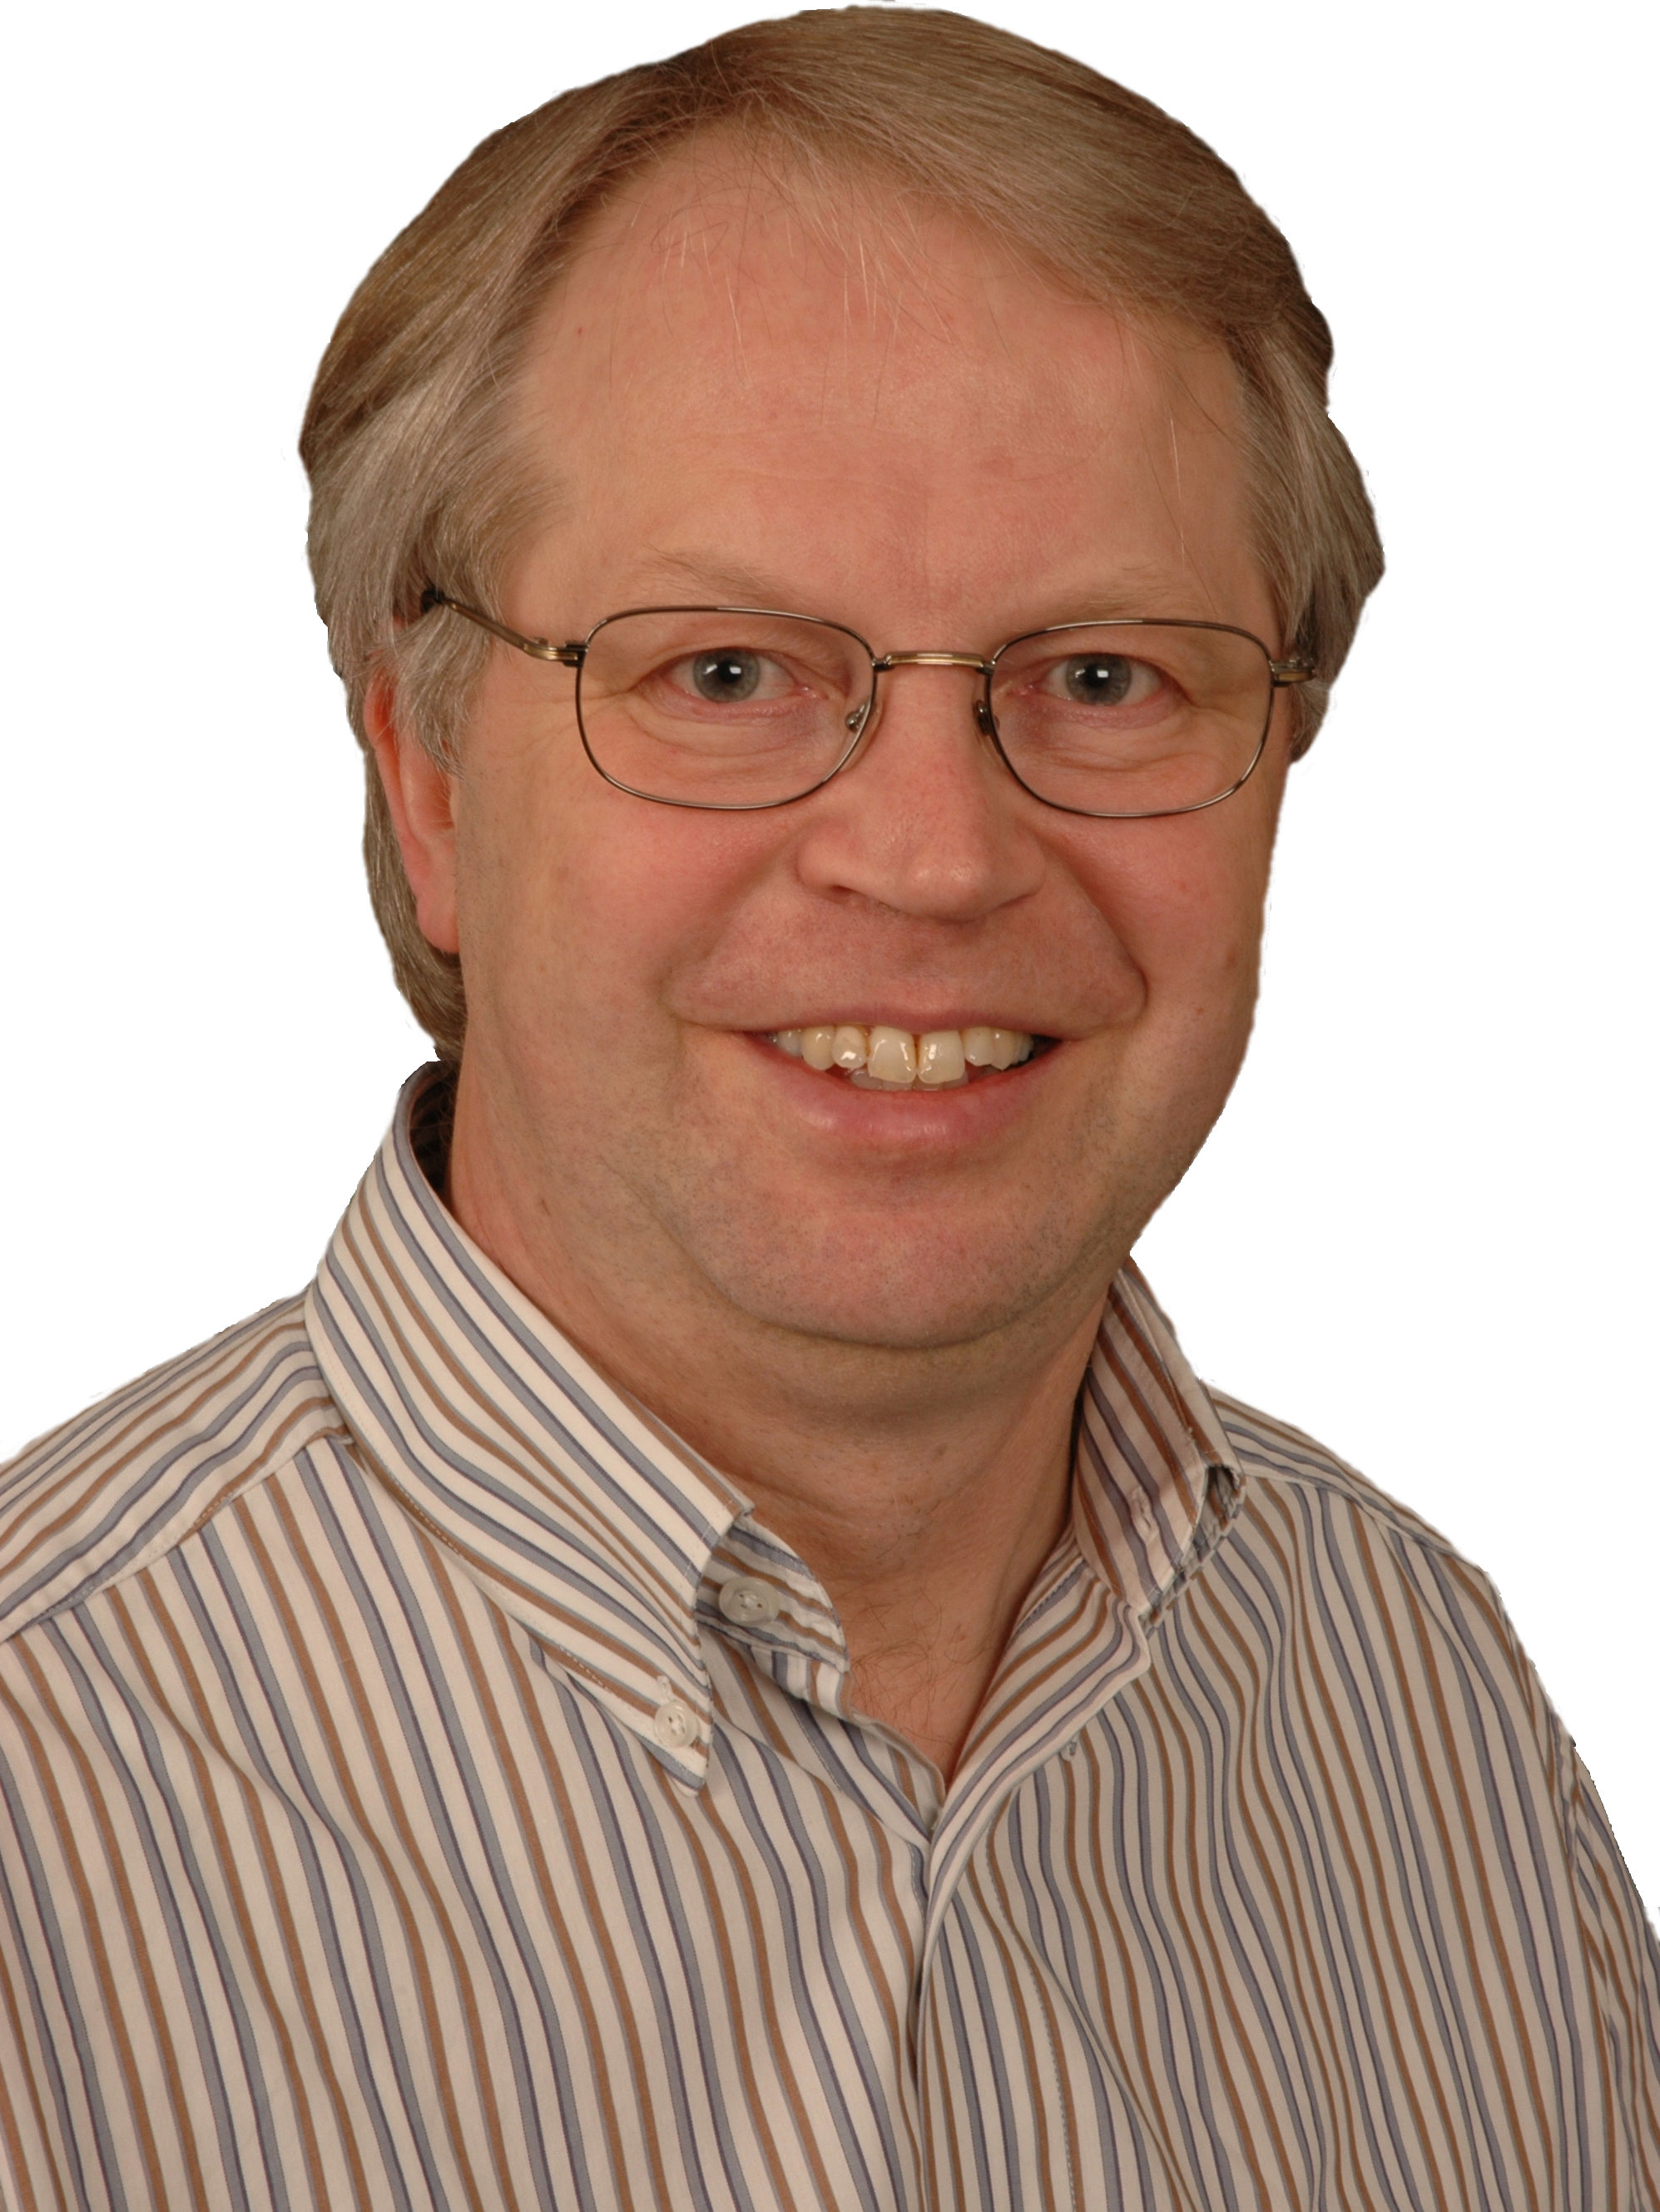
\includegraphics[width=0.7\linewidth]{bilder/dozenten/struck.png}\\
	{Dr. Werner Struckmann}
\end{figure}
Programmiert wird hier fast ausschlie"slich in Java. Wer keine oder nur wenig Erfahrungen mit Java gemacht hat, sollte unbedingt die kleinen "Ubungen bearbeiten.


\subsubsection{Wissenschaftliches Arbeiten}

% \begin{figure}[h]
% 	\centering\includegraphics[width=0.7\linewidth]{bilder/diethelm.png}\\
% 	{Dr. Ira Diethelm}
% \end{figure}
Hier werden Methoden und Richtlinien behandelt, die man zum Erstellen
wissenschaftlicher Arbeiten ben"otigt.

\subsection{Interview mit PD Dr. Bode}

Privatdozent Dr. Bode leitet die großen und kleinen Übungen zur
Vorlesung ,,Diskrete Mathematik für Informatiker''. Er hat sich
freundlicherweise für ein Interview zur Verfügung gestellt.

\nquestion{Was und wo haben Sie studiert?} \\
\nquestion{Welchen Bezug haben Sie als Mathematiker zu Informatik?}\\
\nquestion{Erzählen Sie eine kleine Anekdote aus Ihrem Studium!}\\
\nquestion{Worum geht es in der Veranstaltung ,,Diskrete Mathematik für
Informatiker''? Welche Rolle spielen die Übungen?}\\
\nquestion{Was können Sie den Studierenden für das erste Semester mit
auf den Weg geben?}\\

  \section{Was ihr sonst noch tun solltet}
% !TEX root = ../../1-te.tex

\subsection{Checkliste}
\label{checkliste}
	Hier wird zusammengefasst, was du in den ersten Tagen des Studiums unbedingt erledigen solltest. Wenn du die ToDos auf der Checkliste nach Erledigung abhakst, verlierst du nicht den Überblick und vergisst nichts.
	
\vspace*{0.5cm}
% !TEX root = ../../1-te.tex

\begin{center}
\begin{tabular}{|p{3mm}|l|p{8cm}|c|c|}
\hline \checkmark 
       & \textbf{Todo}             & \textbf{Zu erledigen bis}                                  & \textbf{Seite}               & \textbf{Muss?} \\ 
\hline & BAföG beantragen          & Spätestens Ende \iftoggle{winter}{Oktober}{April}          & \pageref{todobafoeg}         & optional \\ 
\hline & Wohnsitz ummelden         & 1 Woche nach Umzug                                         & \pageref{todoummelden}       & ja \\
\hline & Mailinglisten             & So früh wie möglich                                        & \pageref{mailinglisten}      & ja \\ 
\hline & Studiengrobplanung        & Vor dem Stundenplan bauen                                  & \pageref{grob}               & ja \\
\hline & Auflagen klären           & So früh wie möglich, final: Ende 2. Semester               & \pageref{auflagen}           & nur Master \\ 
\hline & Persönlicher Stundenplan  & Siehe Terminzettel der Fachgruppe                          & \pageref{masterstundenplan}  & ja \\ 
\hline & Prüfungsbogen             & Spätestens \iftoggle{winter}{Dezember}{Mai}                & \pageref{todoanmeldung}      & ja \\ 
\hline & Prüfungsanmeldung         & 12.12.2017 - 11.01.2018, schriftlich oder online           & \pageref{todoanmeldung}      & ja \\ 
\hline & Blog abonnieren           & So früh wie möglich                                        & \pageref{fachgruppe}         & ja \\ 
\hline & Prüfungsordnung lesen     & Zu den ersten Klausuren                                    & \pageref{po}                 & ja \\ 
\hline & TUcard validieren         & Zu Beginn und zu jedem neuen Semester                      & \pageref{tucard}             & ja \\
\hline & Bibliotheksausweis        & Vor der ersten Buchausleihe                                & \pageref{todobib}            & optional \\
\hline & Stud.IP-Nachrichten weiterleiten  & Wenn man nichts verpassen möchte         & \pageref{tumails}            & optional \\
\hline
\end{tabular} 
\end{center}
\tocheck{4}{Exakte Daten Anmeldewoche einfügen, s.\url{https://www.tu-braunschweig.de/fk1/service/informatik/pa}}

\begin{multicols}{2}

\subsubsection{BAföG}
	\label{todobafoeg}

	Wer Studierendenförderung nach dem Bundesausbildungsförderungsgesetz (BAföG) beantragen möchte, sollte sich am besten gründlich informieren. Sehr zu empfehlen ist da: \\
	\verUrl{4}{https://www.xn--bafg-7qa.de/}
 
	Förderungsanträge gibt es zum Download oder in Papierform im EG des Amtes für Ausbildungsförderung in der Wilhelmstraße 1. Wenn du BAföG beantragen möchtest, stelle den Antrag so früh wie möglich, denn es wird nicht rückwirkend gezahlt.

	Zum Anfang des Semester ist mit längeren Wartezeiten zu rechnen, im Notfall kannst du beim AStA-Sozialreferat ein kurzfristiges, zinsloses Darlehen beantragen, um den ersten Monat zu überbrücken. Das Darlehen ist auf 450 Euro begrenzt und muss spätestens nach drei Monaten zurückgezahlt werden. Mehr Informationen findest du auf der Seite des Sozialreferats: \verUrl{4}{https://www.asta.tu-braunschweig.de/referate/sozialreferat/}


\subsubsection{Ummelden}
	\label{todoummelden}

	Wer neu nach Braunschweig gezogen ist, muss sich innerhalb einer Woche beim Einwohnermeldeamt anmelden. Wenn ihr die Frist verpasst, drohen theoretisch Strafen, aber praktisch sieht es da nicht so streng aus. Wenn man Braunschweig als Erstwohnsitz wählt, bekommt man (ein Jahr später) eine einmalige Zuzugsprämie von 100 Euro (Immatrikulationsbescheinigung nicht vergessen). Alternativ kann man Braunschweig auch als Zweitwohnsitz wählen.

\subsubsection{Prüfungsanmeldung}
	\label{todoanmeldung}

	Du musst dich für alle Prüfungen, an denen du teilnehmen willst, vorher beim Prüfungsamt anmelden. Die Fristen sind relativ früh im Semester. Die Termine werden im Laufe des Semesters veröffentlicht (Seiten des P-Amtes (\verUrl{3}{https://www.tu-braunschweig.de/fk1/service/informatik/pa}), Mailingliste). Prüfungen können im Prüfungsanmeldezeitraum schriftlich im Prüfungsamt oder online über das QIS-Portal angemeldet werden.
	Vor deiner ersten Prüfungsanmeldung musst du außerdem ein Datenblatt ausfüllen. Es empfiehlt sich, das bereits vor der Anmeldewoche zu machen, weil die Schlangen dann nicht so lang sind.

	Für die Online-Anmeldung benötigst du eine TAN-Liste, die du dir vorher im Prüfungsamt organisieren musst.

	Unter folgendem Link findest du außerdem alle Prüfungstermine für die Informatik:
	\verUrl{3}{https://www.tu-braunschweig.de/fk1/service/informatik/pa}

\subsubsection{TUcard}
	\label{tucard}
	
	Alle Studierenden der TU erhaten den elektronische Studierendenausweis TUcard, die auch als Bibliotheksausweis und Mensakarte genutzt werden kann.

	Damit die Karte gültig ist, muss sie zu Beginn und zu jedem neuen Semester validiert werden. Das bedeutet, dass der Thermostreifen auf der Karte in einem Validierungsdrucker mit den aktuellen Daten beschrieben wird.

	Das Börsenguthaben der Karte, beispielsweise zum Bezahlen in der Mensa, kann an Börsenaufwertern (auch denen, die sich bereits in den Mensen befinden) aufgeladen werden.

	Zum Drucken kann Guthaben der Karte auf ein Druckkonto umgebucht werden. Dies geschieht an den Druckkontenumbuchern.

	Weitere Informationen zur TUcard findest du unter: \verUrl{3}{https://www.tu-braunschweig.de/studium/imstudium/tucard}

\subsubsection{Uni-Bibliothek}
	\label{todobib}

	Um Bücher in der Uni-Bibliothek ausleihen zu können, brauchst du einen Ausweis. Dieser ist in deiner TUcard integriert. Diesen kannst du an einem der Terminals in der Bibliothek, oder online beantragen und am Schalter freischalten. Je nachdem, ob du zu Beginn schon Bücher brauchst, kannst du die Karte auch später aktivieren.

	In der Bibliothek stehen außerdem Kopierer bereit, die du nutzen kannst. Einen davon kannst du mit Kleingeld befüllen, kompfortabler geht es aber mit einer Kopierkarte. Die bekommst du für ein paar Euro direkt in der Bibliothek. Zu Semesterbeginn gibt es oft noch Einführungskurse in die Bibliotheksbenutzung. Ob du deinen Bibliotheksausweis vor oder nach diesem Kurs aktivierst, ist egal.
	
\end{multicols}

\subsection{Sonstige Informationen}
%TODO raus damit
  \section{Computer und so...}
% !TEX root = ../../1-te.tex

\subsection{Elektronisch informiert}
	\label{elekinf}
	Die wichtigsten Aufgaben der Studierenden sind der Besuch von Lehrveranstaltungen, Zeitmanagement für Studium und Freizeit und Informationsbeschaffung. In diesem Artikel geht es um den letzten Punkt. Da wir nun mal Informatik studieren, soll die Informationsbeschaffung über das Internet erfolgen.

	\subsubsection*{Mailinglisten}
	\label{mailinglisten}
		Die wichtigste Mailingliste für Informatikstudierende ist die Liste \textbf{cs-studs}. Sie ist \emph{die} Informationsquelle. Hier werden Ankündigungen zu Lehrveranstaltungen gemacht, die Fachgruppe kündigt hier Spiele- und Grillabende an und es gibt oft Angebote zu Hiwistellen oder offenen Teamprojekten, Bachelorarbeiten etc. und selbstverständlich ist dies auch ein guter Ort, um Fragen zum Studium loszuwerden.

		Wer längere Diskussionen sucht, kann diese auf der Liste \textbf{cs-studs-discuss} finden bzw. führen. Diese Liste ist noch relativ neu und damit liegt es auch an euch, ihr Leben einzuhauchen.

		Da bei den Wirtschaftsinformatikern oftmals auch informatikrelevante Themen diskutiert werden, lohnt sich möglicherweise auch ein Blick in \textbf{winfo-studs}. 
		Wer an Stellenangeboten und Werbung aus der freien
		Wirtschaft interessiert ist, sollte Mailingliste
		\textbf{firmenkontakt} abonieren. Die
		Informatik-Kolloquien, das sind Vorträge von
		üblicherweise externen Referent/innen zu Informatik-Themen,
		werden auf der Mailingliste \textbf{kolloq} angekündigt.
		Unter
		\verUrl{4}{https://mail.ibr.cs.tu-bs.de/mailman/listinfo/}
		findest du eine umfassende Liste der angebotenen Mailinglisten in der Informatik.

	\subsubsection*{IRC Channel}
		Im Freenode IRC Chat (\verUrl{4}{http://freenode.net}) gibt es den Channel \url{###cs-studs}. Hier sind immer ein paar BraunschweigerInnen und große Teile der Fachgruppe online. Die Gesprächsthemen haben (im weitesten Sinne ;) mit dem Studium zu tun.

	% \subsubsection*{Clevershit}

	% 	Auf jeden Fall einen Besuch wert und eine gute Hilfe bei allem, was das Studium betrifft, ist das von Studierenden ins Leben gerufene Portal \mbox{\verUrl{2}{https://clevershit.de/}}.

	% 	Dieses von Studierenden für Studierende erstellte und geführte Plattform bietet eine gute Anlaufstelle für Fragen jeglicher Art. Es gibt eine Materialsammlung zu allen Veranstaltungen der ersten Semester.

\subsubsection*{Sonstige Informationen}
	\begin{description}
		\item[Allgemeines Vorlesungsverzeichnis:] ~\\
			{\footnotesize\verUrl{4}{http://vorlesungen.tu-bs.de}}
		\item[Uni-Bibliothek:] ~\\
			{\footnotesize\verUrl{4}{http://www.biblio.tu-bs.de}}
		\item[Druckkosten:] ~\\
			{\footnotesize\verUrl{4}{https://www.tu-braunschweig.de/it/service-interaktiv/druckkosten}}
		\item[Don't Panic online] ~\\
			{\footnotesize\verUrl{4}{http://www.tu-braunschweig.de/Medien-DB/it/dontpanic.pdf}}
	\end{description}

\newpage
% !TEX root = ../../1-te.tex

	\subsection{Wozu Computer?}
		\subsubsection{Vorlesungen Online}
			Zu den meisten Vorlesungen kannst du die Skripte im Internet finden. Für einige Vorlesungen gibt es sogar Ton- oder Videomitschnitte.

			Es gibt auch immer engagierte Studierende, die ihre Vorlesungsmitschriften online stellen. Da diese sehr wahrscheinlich in deinem Semester sind, hilft es, wenn du dich in den Vorlesungen umhörst.

		\subsubsection{Organisatorisches ohne Papier}
			Ansonsten gibt es eine Reihe von Informationen, die du vor allem im Internet findest, auch mehr und mehr Formalitäten (zum Beispiel die Prüfungsanmeldung\footnote{\verUrl{6}{https://vorlesungen.tu-bs.de}}) können dort geregelt werden. Desweiteren kannst du dir auf den Webseiten der TU Braunschweig einen individuellen Stundenplan zusammenstellen, in Erfahrung bringen, wann die nächsten Klausuren stattfinden oder das Prüfungsamt geöffnet hat\footnote{\verUrl{6}{https://www.tu-braunschweig.de/fk1/service/informatik/pa}}, lesen, was es in der Mensa zu essen gibt\footnote{\verUrl{6}{http://www.stw-on.de/braunschweig/essen/menus/mensa-1}}, offene HiWi-Stellen bei den Instituten finden\footnote{\verUrl{6}{https://www.tu-braunschweig.de/wirueberuns/stellenmarkt/wen-wir-suchen}} und vieles mehr.

		\subsubsection{Mitschreiben am PC}
			Auf den ersten Blick mag es naheliegen, sich während der Vorlesungen Notizen am Laptop anzufertigen. In der Praxis gibt es da aber eine Reihe von Problemen, vor denen wir  warnen möchten. Es hat schließlich seinen Grund, das nur rund 5\% der Studierenden in der Vorlesung am Laptop sitzen: Die meisten Tafelanschriften bestehen  aus verschachtelten Formeln, fremdartigen Buchstaben und verworrenen Zeichnungen. Diese in Echtzeit in den Laptop einzuhacken ist eine besondere Kunst, die du mit Notepad und Word gar nicht erst probieren brauchst. Eine Chance hast du vielleicht mit einem Tablet oder wenn du \LaTeX{} bereits im Schlaf beherrschst -- aber wer tut das schon zu Beginn des Studiums?

			In den Vorlesungen, in denen du nicht tafelweise abschreiben, sondern nur hier und da mal etwas notieren musst, ist ein PC schon nützlicher. Wenn du ab und zu den Vortrag der bzw. des Profs damit vergleichen möchtest, was er oder sie in das Skript geschrieben hat, kann dir der mitgebrachte Laptop unter Umständen das Ausdrucken von ein paar hundert Seiten ersparen. Du wirst aber schnell merken, dass es in praktisch keinem der Hörsäle und Seminarräume Steckdosen gibt, dir nur begrenzt Platz zur Verfügung steht und einige Profs mit technischen Geräten in der Vorlesung so ihre Probleme haben.

		\subsubsection{Hausaufgaben am PC}
			In vielen Fächern musst du regelmäßig Hausaufgaben erledigen und abgeben. Keiner erwartet von dir, dass diese mit dem PC gemacht werden, manchmal müssen sie sogar handschriftlich sein. Es hat aber auch gewisse Vorteile, sie am Computer zu schreiben (z.B. mittels \LaTeX) und dann auszudrucken.

		\subsubsection{\LaTeX}
			Bei \LaTeX handelt es sich um ein Satzsystem für wissenschaftliche Texte, wie Haus- oder Abschlussarbeiten. Erwähnenswert ist die hervorragende Unterstützung für den Satz mathematischer Formeln und, dass dabei mit Befehlen, ähnlich wie in HTML gearbeitet wird. Es gibt \LaTeX-Kurse\footnote{Angeboten z.B. durch das GITZ: \verUrl{6}{https://www.tu-braunschweig.de/it/dienste/61/6111}},
			 aber mit den Infos im Web kann man sich das auch selbst beibringen. Je eher du damit anfängst, desto weniger Probleme hast du später, wenn du damit z.B. deine Abschlussarbeit aufsetzt.

		\subsection{Computer-Pools an der Uni}
			Es ist immer nützlich zu wissen, wo man mal schnell an einen Computer kann.

			\begin{itemize}
				\item[*] Im Erdgeschoss des Altbaus gibt es auf der rechten Seite zwei Computerräume, einer weiter vorne (\textbf{PK 4.6}) und einer genau in der Ecke des Gebäudes (\textbf{PK 4.5}). Zwei weitere Räume (\textbf{PK 4.8} und die \textbf{Datenstation}) findest du im ersten Stock des Altbaus, auch wieder in der rechten Ecke. Die Rechner in \textbf{PK 4.5} und \textbf{PK 4.8} sind mit Linux ausgestattet.

				\item[*] Reichlich Computer findest du schließlich im Gauß-IT-Zentrum (GITZ) an der Hans-Sommer-Straße. Das ist der gedrungene, fast würfelförmige, dunkle Klotz hinter dem Elektrotechnik-Hochhaus (E-Tower). Hier gibt es mehrere frei zugängliche Räume mit Linux- und Windowsrechnern. Es gibt hier auch Räume für Medienbearbeitung, wo du etwa Video-Digitalisierer, ein Tonstudio und Rechner mit der Adobe Creative Suite nutzen kannst.

				\item[*] Seit 2010 stellt das IBR (Institut für Betriebssysteme und Rechnerverbund) im Raum G40 des Informatikzentrums einen Rechnerraum mit vielen, schnellen Linux-Rechnern  zur Verfügung. Zu diesem CIP-Pool (Computer-Investitions-Programm) bekommt man mit seiner y-Nummer Zutritt. Wenn man Glück hat, funktioniert sogar einer der beiden Drucker in diesem Raum, so dass man zum Drucken nicht das Informatikzentrum (IZ) verlassen muss.
			\end{itemize}

		\subsection{Der eigene Rechner}
			Wenn du trotz aller Widrigkeiten planst, dir extra für dein Studium einen (tragbaren) Rechner anzuschaffen, dann hast du hier gleich ein wenig Kaufberatung: Viel (Rechen- bzw. Grafik-)Leistung brauchst du im Studium  nur für sehr wenige spezielle Fachgebiete -- das einfachste Notebook wird also vermutlich schon reichen. Wichtiger ist vielmehr die Akkulaufzeit und die WLAN-Empfangsstärke.

		\subsubsection{Welches System?}
			Dir wird auffallen, dass zwar alle Systeme geduldet sind, aber dir Linux hier deutlich öfter über den Weg laufen wird als in der freien Wildbahn. Auch wir sind große Linux-Fans und haben deshalb ab Seite \pageref{linux} ein paar Infos dazu zusammengetragen.

			Aber trotz dieser nicht ganz unauffälligen Beeinflussung gilt: Beim Betriebssystem hast du freie Wahl. Sämtliche Software, die du für's Studium brauchen  könntest, gibt es für alle großen Systeme, meist sogar gratis. Für Linux ist eh  praktisch alles frei erhältlich, für Windows spendiert Microsoft den Studierenden auch alles außer Office (siehe Seite \pageref{msdnaa}), und auch Apple bringt dich dank Studierendenrabatte durch Bachelor und Master.
% !TEX root = ../../1-te.tex

\subsection{Gauß-IT-Zentrum}

	Das Rechenzentrum der TU-Braunschweig heißt Gauß-IT-Zentrum oder kurz GITZ. Es bietet dir eine Vielzahl an Diensten an. Manche davon kannst du nur vor Ort nutzen, also in der Hans-Sommer-Str. 65, direkt hinter dem ,E-Tower'. 
	
	Andere Dienste sind auch in den Außenstellen, wie z.B. im
	Altgebäude zu finden und das allermeiste lässt sich über das Netz an der gesamten Uni oder sogar weltweit in Anspruch nehmen.

\subsubsection{GITZ-Account}
\label{todogitz}
	Unser Rechenzentrum, das Gauß-IT-Zentrum, stellt  diverse Dienste zur Vefügung, wovon manche quasi lebenswichtig sind, andere eher nebensächlich. Aber für all diese Dienste brauchst du eine GITZ-Account-Nummer und ein Passwort. Diese so genannte y-Nummer ist nicht das gleiche wie eure Immatrikulationsnummer. In der Regel bekommt man schon vor Semesterbeginn eine Nummer und ein vorläufiges Passwort per Post zugesendet. Dieses Passwort brauchst du dir nicht merken, denn man kann es nur verwenden, um  sich ein richtiges Passwort für die spätere Verwendung auszusuchen. Das sollte man schnellstmöglichst erledigen, da man sonst die Dienste des GITZ (z.B: WLAN, die Pool-Rechner etc) nicht nutzen kann. 
	
	Es kann auch passieren, dass du den besagten Brief vom GITZ  gar nicht bekommst, dann gehst du einfach selbst zum GITZ in die Hans-Sommer-Straße und besorgst dir dort einen. Keine Sorge, das passiert halt ab und zu, ist aber nicht weiter schlimm.

	\subsubsection{Emailadresse}
		Zusammen mit eurem GITZ-Account bekommt ihr auch ein neues Email-Postfach mit bis zu drei Adressen (y00000000@tu-bs.de, vorname.nachname@tu-bs.de, v.nachname@tu-bs.de). Leider kommt es dabei manchmal zu Problemen, also nicht wundern, wenn euch Emails mal mit kleiner Verzögerung erreichen. 

	\subsubsection{WLAN}
		\label{wlan}
		WLAN wird vom Rechenzentrum in vielen Hörsälen (wie dem \textbf{Audimax} und \textbf{SN19.1}), im IZ, in der Universitätsbibliothek (UB), der Mensa und im GITZ angeboten. Notebookbesitzer finden auf folgender Webseite alle notwendigen Informationen, um das \emph{eduroam} nutzen zu können. \verUrl{4}{http://www.tu-braunschweig.de/it/dienste/11/1106}

		Das \emph{eduroam} ist ein international standardisierter Zugang, der an vielen europäischen Hochschulen funktioniert. Einmal eingerichtet kannst du also mit deinen TU-BS-Zugangsdaten problemlos an anderen Unis surfen.

		Die Anleitungen der TU-Braunschweig werden dir nahelegen, eine spezielle Software nachzuinstallieren. Es geht aber für alle aktuellen Betriebssysteme auch ohne, also nur mit Boardmitteln -- um herauszufinden wie, schau einfach im Netz nach, was andere Unis zu \emph{eduroam} zu sagen haben. Für Windows XP (und eng verwandte Versionen) bietet z.B. die Uni Graz eine schöne Anleitung.

		Wer etwas schneller unterwegs sein will (oder wessen Empfang überhaupt nicht ausreicht), dem sei das normale Ethernet ans Herz gelegt. Ein Kabel dazu musst du dir selbst mitbringen. Dosen zum Anschließen gibt es in der Uni-Bibliothek (z.T. versteckt unter runden Klappen im Boden, z.T. an der Fensterseite freiliegend), dem Informatik-Zentrum, sowie einigen Rechnerräumen im Altgebäude und Rechenzentrum.

\begin{multicols}{2}
\subsection{Linux}
	\label{linux}
	Als Informatiker befasst man sich oft mit abstrakten und allgemeinen Konzepten, die unabhängig von konkreten Betriebssystemen gültig sind. Aber sobald man sich an einen Rechner setzt, hat man es dann doch mit einem konkreten System zu tun, und innerhalb der Rechnerpools an der Uni ist dies meist die eine oder andere Linux-Version. Du wirst also im Studium nicht drum herum kommen, etwas Erfahrung damit zu sammeln.

	Auf deinem eigenen Rechner kannst du natürlich machen, was immer du möchtest, aber viele von uns bevorzugen auch dort Linux oder ein anderes Unix-artiges System. Der Umstieg ist gar nicht so schwer wie man denkt bzw. wie er vor 10 Jahren mal war, und dank Live CDs, Dual Boot und Virtualisierung kannst du sogar Linux und dein bisheriges System parallel laufen lassen und somit ganz unverbindlich reinschnuppern.

	\subsubsection{Einstiegshilfen}
		Falls du mit Linux bisher keine Erfahrung hast, könnte der Studienbeginn der passende Zeitpunkt sein. Die Fachgruppe veranstaltet von Zeit zu Zeit Linux-Installationsparties die dir beim Einstieg helfen. Wenn dann im Alltag irgendein Problem auftritt, ist der nächste Linux-Guru meist nur wenige Meter entfernt.

		Auch wenn du nocht nicht 100\% sicher bist, wohin die Reise geht, solltest du also vor dem Kauf eines neuen Rechner sicherheitshalber checken, ob die Hardware Linux-Kompatibel ist.

	\subsubsection{SSH - Zugriff aus der Ferne}
		Um vom heimischen PC aus Zugriff auf deinen Uniaccount zu haben, kannst du von Linux aus ssh benutzen. Für Windowsbenutzer gibt es zwei nette kleine Tools, Putty und WinSCP. Deinen Uniaccount erreichst du über den Server \texttt{rzstudio.rz.tu-bs.de}.

		\begin{description}
			\item[Putty] stellt dir eine Shell auf dem UNIX"~Rechner bereit. Damit kannst du so auf deinem Rechner arbeiten, als würdest du direkt auf dem Server arbeiten (tust du ja auch). Um auch grafische Programme starten zu können, musst du noch einen X"~Server für Windows installieren, z.B. X-Deep32.
			\item[WinSCP] ist ein Tool, das einem FTP"~Client ähnelt. Mit diesem kannst du Dateien von und zu deinem Uniaccount kopieren. Der Vorteil ist, dass die Übertragung verschlüsselt ist und Passwörter somit nicht abgehört werden können.
		\end{description}

		Zu allen in diesem Text angesprochenen und noch zu vielen anderen Computerproblemen mehr gibt es Informationen im Heft \emph{Don't Panic}, das kostenlos im Rechenzentrum erhältlich ist. Nimm es dir gleich mit, wenn du deine y"~Nummer beantragst.

	\subsubsection{Linux-Bezug an der TU-BS}
		Fast alle Linux-Distributionen und Softwarepakete für Linux sind freie Software und somit kostenlos erhältlich.

		Für Studierende mit Breitband-Internetzugang sind vermutlich die diversen Mirror-Server an der Uni interessant. Hier stehen die größeren Distributionen bereit:
	  
		\begin{description}
			\item[\url{ftp://ftp.rz.tu-bs.de/}]~\\Enthält Openoffice-, Mozilla-, Gentoo-, Slackware- und Ubuntumirror, CCC Vorträge
			\item[\url{ftp://debian.tu-bs.de/}]~\\Debian-, Kanotix- und Knoppixmirror
			\item[\url{ftp://ftp.ibr.cs.tu-bs.de/}]~\\Mehr CCC Vorträge, diverse freie Software (größtenteils für Unix/Linux)
		\end{description}

		Für Studierende ohne breitbandigen Netzzugang sind sicherlich die CDs nützlich, die sich jede/r im IT Service-Desk\footnote{http://www.tu-braunschweig.de/it/service-desk} im Gauß-IT-Zentrum, \textbf{Raum 017}, ausleihen kann. Dort stehen eigentlich immer die neusten Versionen von SuSE, Mandrake, Fedora, Gentoo, Debian und Knoppix sowie diverse ältere Distributionen zur Verfügung. Dank eines DVD-Brenners können inzwischen auch --~soweit vorhanden (SuSE, Knoppix)~-- die DVD-Versionen verliehen werden. Auf der sicheren Seite ist, wer vorher einen Abholtermin vereinbart, damit die gewünschte Distribution garantiert greifbar ist: 0531/391-5555.
\end{multicols}
\begin{figure}[h]
  \includegraphics[width=\linewidth]{bilder/comics/stein2}
\end{figure}
\subsection{Microsoft Academic Alliance}
	\label{msdnaa}
	Die TU hat  2003 eine Campuslizenz\footnote{\verUrl{0}{http://msdn.microsoft.com/en-us/default.aspx}} von Microsoft erworben, in deren Rahmen du Microsoftprodukte kostenlos beziehen kannst.\\ 
	Zur Auswahl stehen die meisten Betriebssysteme, Entwicklungswerkzeuge und diverse Serversoftware\footnote{\sloppy Eine komplette Liste der Software findet sich unter \verUrl{0}{http://msdn.microsoft.com/en-us/subscriptions/downloads/default.aspx}}. Die Office-Suite ist explizit \textbf{nicht} enthalten.

	Die Software darf zu nicht-kommerziellen Zwecken in Forschung und Lehre eingesetzt werden, jedoch keine Infrastrukturaufgaben erfüllen\footnote{Die Nutzungsbedingungen sind nachzulesen unter \verUrl{0}{https://www.dreamspark.com/}}. Infos gibt es unter \verUrl{0}{https://www.tu-braunschweig.de/it/service-interaktiv/software/doku/msdn-aa}.

	Du brauchst ein laufendes Windows, um Software (also auch
	Windows selbst) herunterzuladen. Du kannst  bei den Operateuren
	im Rechenzentrum in \textbf{Raum 015} eine Windows-CD gegen eine Schutzgebühr von ca. 10 Euro erwerben, die übrige Software kannst du dort ausleihen oder unter \verUrl{0}{https://www.tu-braunschweig.de/it/service-interaktiv/software/doku/msdn-aa} downloaden.


  \section{Freizeit}
\subsection{Discos}

\begin{description}
\item[Ballhaus] \hfill K"uchenstra"se 1\\
Do -- Sa \hfill 22 -- 4 Uhr\\
Charts, Tanz

\item[Bogey's] \hfill Stecherstra"se\\
Do -- Sa \hfill ab 21 Uhr\\
Deutschrock, Pop, Schlager

\item[Brain Klub] \hfill Bruchtorwall\\
Do -- Sa \hfill ab 23 Uhr\\
Alternative, Funk, HipHop, Independent, Reggae, Soul, Live-Konzerte und DJ-Shows\\
\nurl{http://www.brain-bs.de}

\item[Jolly Joker] \hfill Broitzemer Stra"se 220\\
Di, Fr \& Sa \hfill 22 -- 4.30 Uhr\\
Alternative, Black Music, Charts, RnB, House, Rock. Vier R"aume, Cocktailbar\\
\nurl{http://www.jolly-joker.de}

\item[Meier Music Hall] \hfill Schmalbachstra"se 2\\
Fr \& Sa \hfill 22 -- 5 Uhr\\
Charts, Independent, Pop, Rock\\
\nurl{http://www.meier-music-hall.de}

\item[Merz] \hfill Gieselerstra"se 35\\
Do -- Sa \hfill ab 21 Uhr\\
Alternative, Pop\\
\nurl{http://www.merz-bs.de}

\item[Schwanensee] \hfill Gieselerstra"se 35\\
Fr \& Sa \hfill 23 -- 4 Uhr\\
Classics, House, Soul

\item[Vibe] \hfill Gieselerstra"se 35\\
Fr \& Sa \hfill 21 -- 3 Uhr\\
Black Music, Funk, Soul\\
\nurl{http://www.vibe-bs.de}

\end{description}


\subsection{Kneipen}

\begin{description}

\item[1/4 Nach] \hfill B"ultenweg 89\\
Bietet die M"oglichkeit zum Bier auch noch eine Runde Billiard zu genie"sen.
Campusviertel\\
\nurl{http://www.viertelnach.de}\footnote{Bei Drucklegung hatte die Seite keine Inhalte, aber vielleicht kommt sie ja wieder\ldots}

% Out of Buisness afik ):
%\item[Anno 1826] \hfill Schleinitzstra"se 1

\item[Charly's Tiger] \hfill Wilhelm-Bode-Stra"se 26\\
Jeden Montag alle Men"us zum halben Preis. Sehr empfehlenswert.


\item[Eusebia] \hfill Spielmannstra"se 11\\
Mischung aus Restaurant, Cafe und Kneipe. Zu jeder Tageszeit empfehlenswert.
Campusviertel

\item[Expertise] \hfill Steinbrecherstra"se 31\\
Gem"utliche Spielekneipe mit einer riesigen Auswahl an Brettspielen.

\item[Funzel] \hfill Rebenring 9\\
  %Neue adresse nachgucken!
Hat meistens ziemlich lange auf. Wer es urig mag, wird hier gl"ucklich.
Campusviertel

\item[Herman's Cafe Bar] \hfill Schleinitzstra"se 18\\
Hier gibt es sehr gute Baguettes, die man in angenehmer Atmosph"are genie"sen kann.
Campusviertel\\
\nurl{www.hermans-cafe.de}

\item[Mephisto] \hfill Fallersleber Stra"se 35\\
Gro"se, aber gem"utliche Kneipe.

%\item[Merz, Vibe, Schwanensee] \hfill Gieselerstr. 35\\
%Alle drei mit unterschiedlicher Musik. Gut zum Rocken geeignet.\\
%\nurl{http://www.merz-bs.de}

\item[Michaelishof]~ \hfill Güldenstr. 8a\\
  Kneipe im Wohnheim Michaelishof\\
  Geöffnet: Donnerstags ab 21:00 Uhr\\
  \nurl{http://www.michaelishof.de/kneipe/}
\item[MonkeyIsland]~ \hfill Rebenring 64\\
  Kneipe im Wohnheim Affenfelsen\\
  Regelmäßig wechselndes ,,Bier der Woche'' und eine riesige
  Spielesammlung\\
  Geöffnet: Donnerstags ab 20:00 Uhr\\
  \\\nurl{http://gruppen.tu-bs.de/monkeyisland/}
\item[R.P. McMurphy's Irish Pub] \hfill B"ultenweg 10\\
Gem"utlicher Irish Pub in Sichtweite der Uni.
Campusviertel
 \item[Schunterkino] \small{Bienroder Weg 54}\\
   \normalsize
   Kinoim Wohnheim an der Schunter\\
   Das Kino verfügt über einen echten Projektor und gemützliche
   Bestuhlung.\\
 %Die Kneipe hat neben    günstigen Preisen zwei Kicker, Tischtennis, Dart und einen
  % Billiardtisch zu bieten.\\
   %Viermal im Jahr werden größere Partys veranstaltet.\\
%   Gemützlicher Kinosaal mit  professionelle Technik bei sehr günstigen
%   Eintritt, regelmäßige Themenabende/Konzerte in der Kneipe, viermal im Jahr
%   größere Partys\\
   Kinovorstellungen: Im Semester Dienstags und Donnerstags ab 20:00 Uhr\\
  % Geöffnet: Dienstags, Donnerstags und Freitags ab 20:00 Uhr
   \\\nurl{http://www.schunterkino.de/}\\
 %  \nurl{http://www.schuntille.de/}
 \item[Schuntille] \small{Bienroder Weg 54}\\
   \normalsize
 Die    Kneipe im Wohnheim an der Schunter 
  % Das Kino verfügt über einen echten Projektor und gemützliche
  % Bestuhlung.\\
  hat neben    günstigen Preisen zwei Kicker, Tischtennis, Dart und einen
   Billiardtisch zu bieten.\\
   Viermal im Jahr werden größere Partys veranstaltet.\\
%   Gemützlicher Kinosaal mit  professionelle Technik bei sehr günstigen
%   Eintritt, regelmäßige Themenabende/Konzerte in der Kneipe, viermal im Jahr
%   größere Partys\\
 %  Kinovorstellungen: Im Semester Dienstags und Donnerstags ab 20:00 Uhr\\
   Geöffnet: Dienstags, Donnerstags und Freitags ab 20:00 Uhr
 %  \\\nurl{http://www.schunterkino.de/}\\
   \nurl{http://www.schuntille.de/}
  % \ \\ \\ \\
   \item[Wild Geese] \hfill G"ordelingerstra"se 49\\
Montags gibt es den Pint f"ur Studenten g"unstiger.
Quizabend und Karaoke.\\
\nurl{http://www.wildgeese.de}

\end{description}
\end{multicols}
%	\end{wrapfigure}
%\newpage
\vfill
\begin{center}
  \includegraphics[width=\linewidth]{bilder/comics/uf005633.png}
\end{center}
\newpage
	\begin{multicols}{2}

%%% Local Variables: 
%%% mode: latex
%%% TeX-master: "../../1-te"
%%% End: 

\input{texte/freizeit/raeume}
\subsection{Tagebücher}
\subsubsection{Tagebuch eines 1. Semesters\ldots}

\begin{description}
\item[05:30] Der Quarz-Uhr-Timer mit Digitalanzeige gibt ein zaghaftes "`Piep-Piep"'
von sich. Bevor sich dieses zu energischem Gezwitscher entwickelt, sofort
ausgemacht, aus dem Bett gehüpft. Fünf Kilometer Jogging an der Oker,
mit einem Besoffenen zusammengestoßen, anschließend eiskalt geduscht.
\item[06:00] Beim Frühstück Heise-Online studiert und dabei neueste Patches geladen.
Danach kritischer Blick in den Spiegel, Outfit genehmigt.
\item[07:00] Zur Uni gehetzt. PK 2.2 erreicht. Pech gehabt: erste Reihe schon besetzt.
Niederschmetternd. Beschlossen, morgen doch noch eher aufzustehen.
\item[07:30] Vorlesung, Algorithmen und Datenstrukturen bei Fekete. Keine Disziplin!
Einige Kommilitonen lesen
Sportteil der BZ oder gehen ins "`Viertel Nach"' frühstücken. Alles
mitgeschrieben. Füller leer, aber über die Witzchen des Dozenten mitgelacht.
\item[08:00] Vorlesung, Lineare Algebra, Marten. Verdammt! Extra neongrünen Pulli
angezogen und trotz eifrigem Fingerschnippens nicht drangekommen.
\item[10:45] Nächste Vorlesung. Nachbar verläßt mit Bemerkung "`Sinnlose
Veranstaltung"' den Raum. Habe mich für ihn beim Prof. entschuldigt.
\item[12:00] Mensa Essen II. Nur unter größten Schwierigkeiten
weitergearbeitet, da in der Mensa zu laut.
\item[12:45] In Fachschaft gewesen. Mathe Skript immer noch nicht fertig. Wollte
mich beim Vorgesetzten beschweren. Keinen Termin bekommen. Daran geht die
Welt zugrunde.
\item[13:00] Fünf Leute aus meiner Stuko-Gruppe getroffen. Gleich für drei AG's zur
Klausurvorbereitung verabredet.
\item[13:30] Dreiviertelstunde im Copyshop gewesen und die Klausuren der letzten 10
Jahre mit Lösungen kopiert. Dann Kleine übung: Ältere Semester haben keine
Ahnung.
\item[15:30] In der Bibliothek mit den anderen gewesen. Durfte aber statt der
dringend benötigen 18 Bücher nur vier mitnehmen.
\item[16:00] Große übung. War gut vorbereitet. Hinterher den Assi über seine
Irrtümer aufgeklärt.
\item[18:30] Anhand einschlägiger Quellen die Promotionsbedingungen eingesehen und
erste Kontakte geknüpft.
\item[19:45] Abendessen. Verabredung im "`Dialog"' abgesagt. Dafür Vorlesungen
der letzten paar Tage nachgearbeitet.
\item[23:00] Videoaufzeichnung von "`Relationale Datenbanken 1"' angesehen und im Bett noch den "`Cormen"'
gelesen. Festgestellt, 18-Stunden-Tag zu kurz. Werde demnächst die Nacht
hinzunehmen.
\end{description}
\begin{center}
  \includegraphics[width=\linewidth]{bilder/comics/stein1.png}
\end{center}
\newpage
\subsubsection{Tagebuch eines 11. Semesters\ldots}

\begin{description}
\item[10.30] Aufgewacht! Ach, Kopfschmerzen, übelkeit, zu deutsch: KATER!
\item[10.45] Der linke große Zeh wird Freiwilliger bei der Zimmertemperaturprüfung.
(Arrgh!) Zeh zurück. Rechts Wand, links kalt; Mist, bin gefangen.
\item[11.00] Kampf mit dem inneren Schweinehund: Aufstehen oder nicht - das ist
hier die Frage.
\item[11.30] Schweinehund schwer angeschlagen, wende Verzögerungstaktik an und
schalte Fernseher ein (inzwischen auch schon verkabelt).
\item[12.05] Mittagsmagazin beginnt. Originalton Moderator: "`Guten Tag liebe
Zuschauer Guten MORGEN liebe Studenten."' Auf die Provokation hereingefallen
und aufgestanden.
\item[13.30] In der Cafeteria der Mensa Katharienstraße beim Skat mein Mittagessen
verspielt.
\item[14.30] Im Hermanns hereingeschaut. Geld gepumpt und 'ne Kleinigkeit
gegessen: Bier schmeckt wieder! Kurze Diskussion mit ein paar Leuten über
die letzte Entwicklung auf dem Computerspielemarkt.
\item[15.45] Kurz in der Bibliothek gewesen. Nix wie raus, total von Erstsemestern
überfüllt.
\item[16.00] Fünf Minuten im IZ gewesen. Nichts los! Keine Zeitung, keine
Flugblätter\ldots
\item[17.00] Stammkneipe hat immer noch nicht geöffnet.
\item[18.15] Resigniert im fgraum ne Flasche Mate geholt und die neuste bbt folge gesehen.
\item[19.10] Komme zu spät zum Date mit dem blonden Erstsemester im Eusebia.
Immer dieser Streß!
\item[01.00] Die Kneipen schließen auch schon immer früher\ldots Umzug ins Jolly Joker.
\item[04.20] Tagespensum erfüllt. Das Bett lockt.
\item[05.35] Am Okerufer von Erstsemester über'n Haufen gerannt worden. Hat mich
gemein beschimpft.
\item[06.45] Bude mühevoll erreicht. Insgesamt \EUR{27,50} ausgegeben. Mehr hatte der
Kleine nicht dabei.
\item[07.05] Schlucke schnell noch ein paar Alkas und schalte kurz das Radio ein.
Stimme des Sprechers: "`Guten Morgen liebe Zuhörer, gute NACHT liebe
Studenten."'
\end{description}

\input{texte/freizeit/sudokus}
  \section{N"utzliches}
\begin{multicols}{2}
\subsection{Semesterticket}
	Euer Studentenausweis berechtigt euch zur Fahrt auf vielen Zugstrecken in Niedersachsen. Unten seht ihr den Gültigkeitsbereich des Semestertickets im Großraum Hannover. Nach Norden und und Westen deckt das Semesterticket weitere Strecken ab. Einen grober Überblick gibt die nebenstehende Karte. 

	Es d"urfen nur Regionalexpress (RE) und Regionalbahn (RB) der Deutschen Bahn AG, sowie teilweise der Metronom in der zweiten Klasse benutzt werden. Also NICHT Strecken der Nordwestbahn (NWB). Einen genauen Überblick findet ihr in Form einer Streckenliste auf der Seite \pageref{streckenliste1}.

	Mehr Details könnt ihr den Seiten des AStA unter \url{http://www.asta.tu-bs.de/semesterticket.php} bzw. \url{http://tinyurl.com/3gn8fhg} entnehmen.
\end{multicols}
\newpage
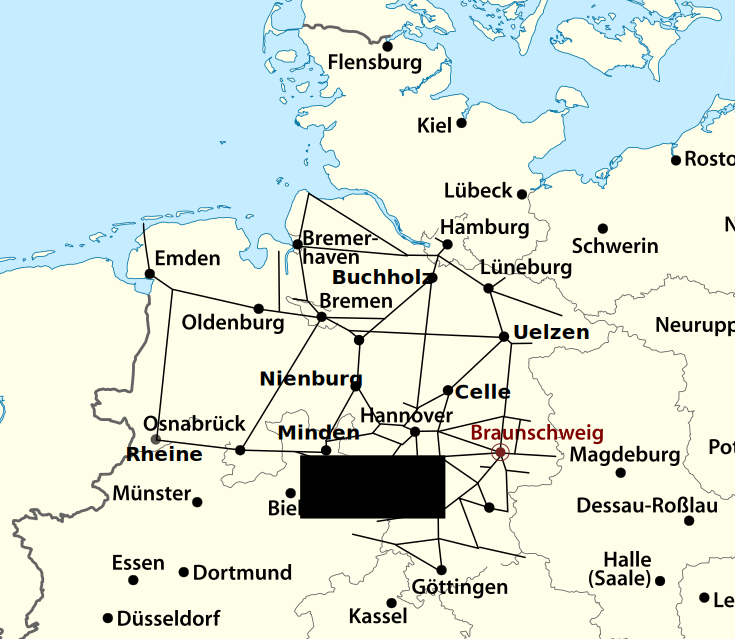
\includegraphics[width=\columnwidth]{bilder/ticket_deutschland.png}
\newpage
\includegraphics[width=\textwidth]{bilder/ticket_bis_11_Dezember.jpg}
\newpage
%\newpage
%\begin{table}[htbp]
Streckenübersicht Wintersemester 2010/2011 und Sommersemester 2011 gültig ab 1.10.2010

\enlargethispage{0.5cm} 
 
%  \begin{addmargin}{-1.5cm}
%\begin{center}
\begin{tabular}{|l|l|l|p{2cm}|}
\hline
\multicolumn{3}{|l|}{\textbf{Strecke/ Streckenabschnitt}}& \textbf{KbN}\\
\textbf{\textit{von}} & \textit{über} & \textbf{\textit{bis}} & \\ \cline{ 1- 4}
Lüneburg &  & Dannenberg Ost & 112 \\ \hline
Braunschweig Hbf & Gifhorn & Uelzen & 115 \\ \hline
Bremen Hbf & Soltau & Uelzen & 116 \\ \hline
Hamburg-Harburg &  & Stade & 121 \\ \hline
Buchholz (Nordheide) & Soltau & Bennemühlen & 123 \\ \hline
Minden Westf. & Nienburg & Rotenburg/Bremen Hbf & 124 \\ \hline
Bremen Hbf &  & Cuxhaven & 125 \footnotemark[1] \\ \hline
Bremen Hbf &  & Bremen-Vegesack & 126 \footnotemark[1] \\ \hline
Echem &  & Lüneburg & 145 \\ \hline
Hannover Hbf & Gifhorn & Wolfsburg Hbf & 300 \\ \hline
Braunschweig Hbf &  & Wolfsburg Hbf & 301 \\ \hline
Uelzen &  & Schnega & 305 \\ \hline
Hannover Hbf & Braunschweig Hbf & Helmstedt & 310 \\ \hline
Braunschweig Hbf & Wolfenbüttel & Schöppenstedt & 312 \footnotemark[2] \\ \hline
Braunschweig Hbf &  & Hildesheim Hbf & 313 \\ \hline
Hannover Hbf & Hildesheim Hbf/Goslar & Bad Harzburg & 320 \\ \hline
Braunschweig Hbf &  & Sz-Lebenstedt & 352 \\ \hline
Braunschweig Hbf & Wolfenbüttel/Vienenburg & Goslar & 353 \\ \hline
Holzminden & Kreiensen & Bad Harzburg & 354 \\ \hline
Ottbergen & Bodenfelde & Göttingen & 356.1 \\ \hline
Ottbergen & Bodenfelde & Northeim & 356.2 \\ \hline
Göttingen & Northeim & Walkenried & 357 \footnotemark[1] \\ \hline
Braunschweig Hbf & Seesen & Herzberg (Harz) & 358 \\ \hline
Haste & Hannover Hbf/Haste & Minden (Westf) & 360.1 \\ \hline
Nienburg (Weser) & Hannover Hbf & Haste & 360.2 \\ \hline
Hannover Hbf & Lehrte & Hildesheim Hbf & 360.3 \\ \hline
Bennemühlen & Hann./Sarstedt & Hildesheim Hbf & 360.4 \\ \hline
Bad Pyrmont & Hameln/Weetzen & Hannover-Flughafen & 360.5 \\ \hline
Celle & Lehrte & Hannover Hbf & 360.6.7 \\ \hline
Hannover Hbf &  & Hannover Bismarckstr. & 361 \footnotemark[1] \\ \hline
Hannover Hbf &  & Löhne (Westf.) & 370 \\ \hline
Löhne (Westf.) & Hameln & Hildesheim Hbf & 372 \\ \hline
Hildesheim Hbf &  & Bodenburg & 373 \\ \hline
Salzbergen & Osnabrück Hbf & Minden (Westf.) & 375 \footnotemark[1] \\ \hline
Bremen Hbf &  & Hannover Hbf & 380 \\ \hline
Osnabrück Hbf &  & Bremen Hbf & 385 \footnotemark[1] \\ \hline
Norddeich Mole & Oldenburg (Oldb) & Bremen Hbf & 390 \footnotemark[1] \\ \hline
Norddeich Mole & Meppen & Rheine & 395 \footnotemark[1] \\ \hline
Emden Hbf &  & Emden Außenhafen & 396 \\ \hline
Leer (Ostfr.) &  & Weener & 397 \\ \hline
\end{tabular}

\footnotetext[1]{nur in den Zügen der DB Regio AG, also nicht in Zügen der Nordwestbahn}
\footnotetext[2]{gültig auch in Bus von  Schöppenstedt-Schöningen-Helmstedt}
%\end{tabular}
%  \end{addmargin}
\label{streckenliste1}
%\end{table}
%\begin{table}[htbp]

%\newpage
%Streckenübersicht Wintersemester 2010 gültig bis 11.12.2010
%
%  \begin{addmargin}{-1.5cm}
%\begin{tabular}{|l|l|l|p{1cm}|}
%\hline
%\multicolumn{3}{|l|}{\textbf{Strecke/ Streckenabschnitt}}& \textbf{KbN}\\
%\textbf{\textit{von}} & \textit{über} & \textbf{\textit{bis}} & \\ \cline{ 1- 4}
%Lüneburg &  & Dannenberg Ost & 112 \\ \hline
%Braunschweig Hbf & Gifhorn & Uelzen & 115 \\ \hline
%Bremen Hbf & Soltau & Uelzen & 116 \\ \hline
%Bremen Hbf &  & Rotenburg/W. & 120 * / *** \\ \hline
%Hamburg-Harburg &  & Stade & 121 \\ \hline
%Buchholz (Nordheide) & Soltau & Bennemühlen & 123 \\ \hline
%Minden Westf. & Nienburg & Rotenburg/Bremen Hbf   & 124 \\ \hline
%Bremen Hbf &  & Cuxhaven & 125 \\ \hline
%Bremen Hbf &  & Bremen-Vegesack & 126* \\ \hline
%Echem &  & Lüneburg & 145 \\ \hline
%Hannover Hbf & Gifhorn & Wolfsburg Hbf & 300 \\ \hline
%Braunschweig Hbf &  & Wolfsburg Hbf & 301 \\ \hline
%Uelzen &  & Schnega & 305 \\ \hline
%Hannover Hbf & Braunschweig Hbf & Helmstedt & 310 \\ \hline
%Braunschweig Hbf & Wolfenbüttel & Schöppenstedt & 312 ** \\ \hline
%Braunschweig Hbf &  & Hildesheim Hbf & 313 \\ \hline
%Hannover Hbf & Hildesheim Hbf/Goslar & Bad Harzburg & 320 \\ \hline
%Braunschweig Hbf &  & Sz-Lebenstedt & 352 \\ \hline
%Braunschweig Hbf & Wolfenbüttel/Vienenburg & Goslar & 353 \\ \hline
%Holzminden & Kreiensen & Bad Harzburg & 354 \\ \hline
%Ottbergen & Bodenfelde & Göttingen & 356.1 \\ \hline
%Ottbergen & Bodenfelde & Northeim & 356.2 \\ \hline
%Göttingen & Northeim & Walkenried & 357 * \\ \hline
%Braunschweig Hbf & Seesen & Herzberg (Harz) & 358 \\ \hline
%Haste & Hannover Hbf/Haste & Minden (Westf) & 360.1 \\ \hline
%Nienburg/Weser & Hannover Hbf & Haste (Han) & 360.2 \\ \hline
%Hannover Hbf & Lehrte & Hildesheim Hbf & 360.3 \\ \hline
%Bennemühlen & Hann./Sarstedt & Hildesheim Hbf & 360.4 \\ \hline
%Bad Pyrmont & Hameln/Weetzen & Hannover-Flughafen & 360.5 \\ \hline
%Celle & Lehrte & Hannover Hbf & 360.6.7 \\ \hline
%Hannover Hbf &  & Hannover Bismarckstr. & 361 * \\ \hline
%Hannover Hbf &  & Löhne (Westf.) & 370 \\ \hline
%Löhne (Westf.) & Hameln & Hildesheim Hbf & 372 \\ \hline
%Hildesheim Hbf &  & Bodenburg & 373 \\ \hline
%Salzbergen & Osnabrück Hbf & Minden (Westf.) & 375 * \\ \hline
%Bremen Hbf &  & Hannover Hbf & 380 \\ \hline
%Osnabrück Hbf &  & Bremen Hbf & 385 \\ \hline
%Norddeich Mole & Oldenburg (Oldb) & Bremen Hbf & 390 * \\ \hline
%Nordenham &  & Bremen Hbf & 391 \\ \hline
%Norddeich Mole & Meppen & Rheine & 395 \\ \hline
%Emden Hbf &  & Emden Außenhafen                     & 396 \\ \hline
%Leer (Ostfr.) &  & Weener & 397 \\ \hline
%\end{tabular}
%\enlargethispage{1cm}
%
%\textbf{* nur in den Zügen der DB Regio AG ** gültig auch in Bus von
%  Schöppenstedt-Schöningen-Helmstedt KbN Kursbuch-Nr}
%\end{tabular}
%  \end{addmargin}
%\label{streckenliste2}
%\end{table}

% Local Variables: 
% mode: latex
% TeX-master: "../../1-te"
% End: 

\documentclass[border=0pt]{standalone}

\usepackage[utf8]{inputenc}
\usepackage{graphicx}
\usepackage{amssymb}
\usepackage[T1]{fontenc}
\usepackage{multicol}
\usepackage{comment}
\usepackage[ngerman]{babel}
\usepackage{wrapfig}
\usepackage[babel,german=quotes]{csquotes}
\usepackage{todonotes}
\usepackage{etoolbox}
\usepackage{sectsty}
% Toggles between winter term and summer term 
\newtoggle{winter}

% This system is meant to make updating the Erste for the new semster simple. Every semster gets a new version number that is larger than the previous one (assigned in config.tex). 
% By using \tocheck, defined below, todos can be left in the source and disabled one by one by incresing the version number of the tocheck. Once all todos are adressed, the new version can be released. Later all todos can be enabled again by incrementing the version number.
\newcounter{version}

% Defines a conditional todo. 2 mandatory arguments:
% 1st param, Valid to version: This todo has been adressd as of the given version
% 2nd param, Todo description: What needs to be done to adress this todo
\newrobustcmd{\tocheck}[2]{
	\ifnumless{#1}{\value{version}}{
		\todo[inline]{#2}
	}{}
}

% Versioned url. 2 mandatory arguments:
% 1st param, Valid to version: This url is still valid as of version
% 2nd param, URL: The url
\newrobustcmd{\verUrl}[2]{\ifnumless{#1}{\value{version}}{\todo[inline]{Check \url{#2}}}{}\url{#2}}
\newrobustcmd{\verHref}[4][]{\ifnumless{#2}{\value{version}}{\todo[inline]{Check \url{#3}}}{}\href[#1]{#3}{\nolinkurl{#4}}}

\newrobustcmd{\FginfoUrl}[0]{https://fginfo.tu-braunschweig.de}
\newrobustcmd{\fginfoUrl}[0]{\verUrl{8}{https://fginfo.tu-braunschweig.de}}

%%

\newrobustcmd{\xkcd}[2]{
	\begin{center}
		\includegraphics[#1]{bilder/XKCD/#2}
	\end{center}
}


% creates a blank page

\newcommand{\blankpage}{
	\newpage
	\thispagestyle{empty}
	\mbox{}
	\newpage
}


% creates a stundenplan
\newenvironment{stundenplan}[6]{%
	\newcommand{\wTag}{#1/6}%
	\newcommand{\hPlan}{#2}%
	\newcommand{\hAbendHeader}{.5}%
	\newcommand{\hAbend}{1.6}%
	\newcommand{\tStart}{zeit(#3,#4)}%
	\newcommand{\tEnde}{zeit(#5,#6)}%

	\pgfmathdeclarefunction{zeit}{2}{\pgfmathparse{##1 + ##2 / 60}}%
	\pgfmathdeclarefunction{tmpYZeit}{1}{\pgfmathparse{-\hPlan * (##1-\tStart) / (\tEnde-\tStart)}}%
	\pgfmathdeclarefunction{yZeit}{1}{\pgfmathparse{%
		max(min(tmpYZeit(##1), tmpYZeit(\tStart)), tmpYZeit(\tEnde)-\hAbendHeader-\hAbend)%
	}}%

%
	\tikzset{%
	  termin/.style={%
	   anchor=north west,%
	   align=left,%
	   %execute at begin node=\setlength{\baselineskip}{1.2em}%
	  }%
	}%

	\newcommand{\tNode}[2]{%
		\node [termin] at (TERMIN) {%
			\begin{varwidth}{1cm*\wTag - .2cm}%
			##1\\%
			\scriptsize ##2%
			\end{varwidth}%
		};%
	}%

%
	\newcommand{\Termin}[8]{%
		%1: Beschreibung, 2: Ort, 3: Tag, 4: Start Stunde, 5: Start Minute, 6: Ende Stunde, 7: Ende Minute, 8: Farbe %
		\draw [##8](\wTag * ##3,{yZeit(zeit(##4,##5))}) coordinate (TERMIN) rectangle (##3  * \wTag + \wTag,{yZeit(zeit(##6,##7))});%
		\tNode{##1}{##2}%
	}%

	\newcommand{\termin}[8]{%
		%1: Beschreibung, 2: Ort, 3: Tag, 4: Start Stunde, 5: Start Minute, 6: Ende Stunde, 7: Ende Minute, 8: Farbe (Fügt Zeit automatisch in Beschreibung ein)%
		\Termin{##1}{##4:##5 -- ##6:##7\ifstrempty{##2}{}{, ##2}}{##3}{##4}{##5}{##6}{##7}{##8}%
	}%

	\newcommand{\abendtermin}[4]{%
		%1: Beschreibung, 2: Ort, 3: Tag, 4: Farbe%
		\draw [##4](\wTag * ##3,-\hPlan-\hAbendHeader) coordinate (TERMIN) rectangle (##3  * \wTag + \wTag, -\hPlan-\hAbendHeader-\hAbend);%
		\tNode{##1}{##2}%
	}%
	\begin{tikzpicture}[font=\small]%
	% spalten
	\foreach \x in {0,...,5}{
		\draw (\x*\wTag,0) -- (\x*\wTag,-\hPlan);
		\draw (\x*\wTag,-\hPlan-\hAbendHeader) -- (\x*\wTag,-\hPlan-\hAbendHeader-\hAbend);
	}
	\draw (6*\wTag,0) -- (6*\wTag,-\hPlan-\hAbendHeader-\hAbend);

	\draw (0,0)--(6*\wTag,0);
	\draw (0, -\hPlan) coordinate (ABEND) rectangle (5*\wTag, -\hPlan-\hAbendHeader);
	\node [anchor=north west,align=center,minimum width=5cm*\wTag] at (ABEND) {\scriptsize \emph{Abend}};
	\draw (0, -\hPlan-\hAbendHeader-\hAbend)--(6*\wTag, -\hPlan-\hAbendHeader-\hAbend);

	\node [anchor=south] at (.5* \wTag,0) {\textbf{Montag}};
	\node [anchor=south] at (1.5* \wTag,0) {\textbf{Dienstag}};
	\node [anchor=south] at (2.5* \wTag,0) {\textbf{Mittwoch\vphantom{g}}};
	\node [anchor=south] at (3.5* \wTag,0) {\textbf{Donnerstag}};
	\node [anchor=south] at (4.5* \wTag,0) {\textbf{Freitag}};
	\node [anchor=south] at (5.5* \wTag,0) {\textbf{Wochenende\vphantom{g}}};
}{\end{tikzpicture}}

\renewcommand{\familydefault}{\sfdefault}

%\clubpenalty = 10000
%\widowpenalty = 10000 
%\displaywidowpenalty = 10000

% Trennregeln
\hyphenation{
	AStA
	Mit-be-wohnerIn-nen
	Pro-fessorInnen
	erwischt
	viiieel
	y-Nummer
	Uniaccount
}

% left aligned sections
%\allsectionsfont{\raggedright}


\settoggle{winter}{true}
\setcounter{version}{6}


\usepackage{nexus}

% supress footnotes
\renewcommand{\footnote}[2][1]{  }
\newcommand{\footref}[1]{  }

\pagestyle{empty}
\tikzset{fgTermin/.style={fill=green!30}}
\tikzset{uniTermin/.style={fill=blue!30}}
\tikzset{vlTermin/.style={fill=red!30}}

\begin{document}
\input{texte/stundenplan/woche\woche.tex}
\end{document}

\documentclass{article}
\usepackage[utf8x]{inputenc}
\usepackage[ngerman]{babel}
\usepackage{eurosym}

\title{Studiengebühren -- eine abschließende Betrachtung}
\author{Henning Günther}
\date{}
\begin{document}
\maketitle

Wir schreiben das Wintersemester 2008/09.
Der Widerstand gegen Studiengebühren liegt in Trümmern.
Nach den vernichtenden Niederlagen im voll\-stän\-di\-gen Boykott der Studiengebühren im Sommersemster 2007, an dem nur 504 der über 14.000 Studenten teilnahmen und dem darauf folgenden, kaum noch spürbaren "`5€"'-Boykott im Wintersemester 2007/08 sind die Studenten kaum noch zu Widerstand bereit.
Im Sommersemster 2008 war das Werk vollbracht, jeder anfängliche Widerstand in alle Winde zerstreut, die anfänglich so breit erscheinende Front der Studiengebührengegner zerschlagen.

Was war geschehen?
Wie konnte sich die vormals so rebellische Studentenschaft, die früher keine Möglichkeit ausließ, gegen das Unrecht zu protestieren, innerhalb von nur einem Jahr in einen in gedemütigter Haltung die Gebühren entrichtenden Haufen Elend verwandeln?

Es hat den Anschein, dass die diabolisch geniale Saat der Studiengebühren-Fürsprecher, die Daumenschrauben der "`Campus-Maut"' nicht sofort und im vollen Umfang anzuziehen, auf ganzer Linie aufgegangen sei.
Denn es traf zunächst die, die sich am wenigsten wehren konnten:
An Erstsemestern die, da noch nicht eingeschrieben, keinen Boykott wagen konnten wurde zuerst erprobt, ob 500€ ein Preis waren, für den die Studenten zu kämpfen bereit wären.
Sie waren es nicht.
Zwar waren viele "`im Prinzip"' dagegen, taten diese Meinung aber nur mäßig auf den wenigen Demonstrationen kund.

Die meisten der Studenten scheinen sich inzwischen mit dem Fakt, mit jährlich 1000€ weniger auskommen zu müssen, abgefunden zu haben.
Kaum jemand gibt sich noch dem Wunschtraum hin, größere Teile der Studenten für irgendeine Form des organisierten Protest zu begeistern.
Es scheint fast als könnten die Studiengebührenschergen bald wieder Morgenluft wittern und in der Lage sein, dank mangelnden Widerstand, ihre kühnsten Träume zu verwirklichen: 1000€ Studiengebühren pro Semester und mehr.

Was wird die Zukunft bringen?
Werden die Besiegten weiterhin wie die Gespenster einer längst vergangenen Zeit durch die Unigänge huschen, von einer Vorlesung zur nächsten hetzen, um sich durch ein schnelleres Studium vielleicht ein paar Euro Studiengebühren zu sparen und gelernt haben, stets mit der Angst vor einer Erhöhung der Gebühren zu leben?
Es bleibt zu hoffen dass den Advokaten des Bezahlstudiums dieser Triumph nicht gewährt wird.

\end{document}


\end{document}

